\setchapterpreamble[u]{\margintoc}
\glsresetall % reset glossary
\chapter{Optimizing modular structures}
Introduction
\todo{change $N_T$ con $N_\text{T}$ }
\todo{NO CELLS}
\todo{metti slend min sulle barre}
\todo{tables always small}
\section{Formulation of a modular structure optimization algorithm}
Assembled modular ultralight structures present an opportunity to greatly improve the performance and cost efficiency of modern aerostructures~\sidecite{cramer_elastic_2019}. The repetitive nature brings various interesting features among which reduced tooling, fast assembly, and short repair time. Additionally, as the mechanical performance of the structure is greatly influenced by the topology and the materials of the repetitive pattern, modular structures are naturally prone to optimization.

In the structure optimization field periodic materials are often modeled by means of asymptotic homogenization~\sidecite{zhou_design_2008}. The heterogeneous module topology (also called \gls{rve}) is treated as homogeneous material with associated mechanical properties \ie equivalent elastic tensor, shear modulus, etc. The homogenization approach is valid only if the \gls{rve} contains enough information about the heterogeneous material and if the structure presents significant periodicity~\sidecite{kalamkarov_asymptotic_2009,li_anisotropic_2020}. When designing modular structures (and not materials), no scale separation is assumed between the repetitive pattern and the structure itself. Consequently, the hypotheses of asymptotic homogenization are not always verified. For that reason, full-scale approaches~\sidecite{wu_topology_2021} have been developed.

\subsection{Variable linking}
\begin{figure*}
    \centering
    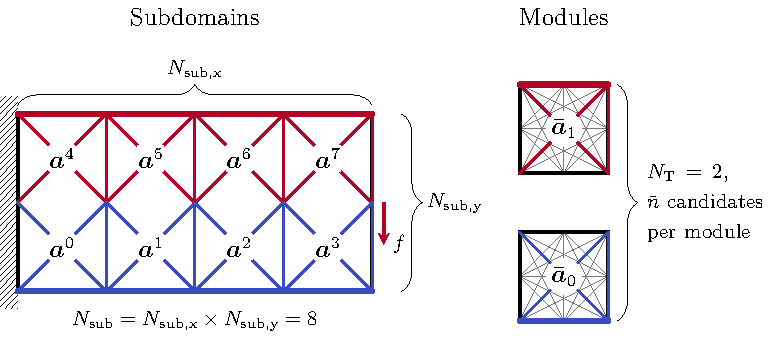
\includegraphics{figures/05_cellular_opt/00_modules_VL_bc/modules_bc.pdf}
    \caption{Notations used for the definition of the variable linking approach used to apply the modularity constraints.}
    \label{fig:05_VL}
\end{figure*}

The variable linking approach~\sidecite{zhang_scale-related_2006} is a full-scale technique that involves first dividing a structure into several subdomains, which are connected during the optimization process \ie subdomains that belong to the same module all share the same cross-sectional areas. The primary goal is to make the manufacturing phase simpler and more efficient, allowing to assemble big structures starting from smaller repetitive modules. With this approach, the optimization perspective shifts. The optimizer design space using the variable linking approach is restricted to the optimization of the topology of the modules, using the whole structure just to impose the necessary mechanical constraints.

We use \figref{fig:05_VL} to illustrate the notation employed in this thesis for modular structures. On the left-hand side of the image, we have the whole test case that we aim to optimize, which is already divided into $N_\text{sub}$ subdomains. Each of these subdomains is bound to exhibit the topology of one of the $N_\text{T}$ module topologies presented on the right side of the image. It is assumed that each module has the same external shape and the identical ground structure used for discretizing the module volume. Within this framework, $\bar{n}$ represents the number of candidate bars in one module, and if we assume a fully connected mesh, we can define $\bar{n} = \bar{m} \cdot (\bar{m}-1)/2$, where $\bar{m}$ stands for the number of nodes in the module. Consequently, for the overall structure, we can write the relationship $N_{\text{el}} = N_{\text{sub}}\bar{n}$.

The vector that holds all the cross-sectional areas of the modules is represented by $\bar{\vect{a}}$, and it belongs to the set of positive real numbers $\mathbb{R}_+^{N_T \cdot \bar{n}}$. This vector is essentially a grouping of individual cross-sectional areas $\bar{\vect{a}}_t$ for each of the $N_T$ modules. In mathematical terms, $\bar{\vect{a}}$ is defined as follows:
\begin{equation}
    \bar{\vect{a}} :=  \{ \bar{\vect{a}}_t \in \mathbb{R}_+^{\bar{n}} \;|\; \forall t \in [1,\dots,N_T]\}
\end{equation}

The topology of the entire structure $\vect{a}$, which originates from the submodules' topology $\bar{\vect{a}}$, is defined as follows:
\begin{equation}
    \vect{a} :=  \{\vect{a}^j \;|\; \forall j \in [1,\dots,N_{\text{sub}}]\}
\end{equation}
and is evaluated using:
\begin{equation}
    \vect{a} = \sum_{t=1}^{N_T} \vect{G}_t\otimes\bar{\vect{a}}_t = \sum_{t=1}^{N_T} \begin{bmatrix}
        h_{1,t} \: \bar{\vect{a}}_t \\
        \vdots\\
        h_{N_{\text{sub}},t} \: \bar{\vect{a}}_t 
        \end{bmatrix}
        \label{eq:05_VL}
\end{equation}
where the $\otimes$ operator represents the Kronecher product and $\vect{h}_{t}$ is the $t$-th column of the mapping matrix $\matr{H} = [\vect{h}_0,\dots,\vect{h}_{N_T}] \in \mathbb{B}^{N_{\text{sub}},N_T}$, where $\mathbb{B}=\lbrace 0,1 \rbrace$ is the Boolean domain. $G_{j,t}$ is the element at the $j$-th row and $t$-th column of the matrix $\matr{H}$. The mapping matrix $\matr{H}$ indexes are defined as follows:
\marginnote{In the case of the structure shown in \figref{fig:05_VL} we have:
\begin{equation}
    \matr{H}=
\begin{bNiceMatrix}[first-row,last-col]
    \scriptstyle\textcolor{axis_gray}{t=0} &\scriptstyle\textcolor{axis_gray}{t=1}&  \\
    1 & 0 & \scriptstyle\textcolor{axis_gray}{\,j=0} \\
    1 & 0 & \scriptstyle\textcolor{axis_gray}{\,j=1} \\
    1 & 0 & \scriptstyle\textcolor{axis_gray}{\,j=2} \\
    1 & 0 & \scriptstyle\textcolor{axis_gray}{\,j=3} \\
    0 & 1 & \scriptstyle\textcolor{axis_gray}{\,j=4} \\
    0 & 1 & \scriptstyle\textcolor{axis_gray}{\,j=5} \\
    0 & 1 & \scriptstyle\textcolor{axis_gray}{\,j=6} \\
    0 & 1 & \scriptstyle\textcolor{axis_gray}{\,j=7} 
\end{bNiceMatrix}
\end{equation}
as the lower submodules (numbered from 0 to 3) exhibit the topology of module $t=0$, while the upper submodules (numbered 4 to 7) the topology of module $t=1$.}
\begin{equation}
    G_{j,t} =
    \begin{cases}
      1 & \text{if the $j$-th subdomain presents the topology of the $t$-th module,} \\
      0 & \text{otherwise.} 
    \end{cases}
\end{equation}
Lastly, we introduce some notation to denote specific bars within the modules and subdomains. We represent the cross-sectional area of the $i$-th bar of the $t$-th module as $\bar{\vect{a}}_{t,i}$, while the cross-sectional area of the $i$-th bar of the $j$-th subdomain as $\vect{a}^j_i$.
\subsection{Topological buckling of modular structures}
Addressing topological buckling in modular structures is a more complex task compared to monolithic structures. This complexity arises from the fact that we must not only consider bars within a single module's design space but also those connecting different modules. Since the nature of this problem heavily relies on how the modules are arranged within the structure, we have opted for a simplification. We focus only on the assessment of nodal instability within each module, modifying the length $\ell^*$ used to evaluate the critical buckling force of \eqrefnotext{eq:04_buck} and \eqref{eq:04_chain_len} only of compressive chains of bars that fall inside a module. Additionally, \eqref{eq:04_side_cons_chain} is modified as follows:
\begin{equation}\label{eq:05_side_cons_chain_modular}
    \bar{\vect{a}}_{t,r} \geq \bar{a}_{t,r=1} \quad r \in \mathcal{C}_{l,r}(\bar{\vect{a}}_t) \quad \forall t \in [1,\dots,N_T].
\end{equation}
We have made this choice knowing that the high connectivity of modular structures tends to reduce the occurrence of nodal instability within the structure. Any potential nodal instability in compressive chains at the structure level is addressed in a subsequent post-processing phase.

\subsection{Optimization formulation}
Monolitic fomulation \ref{eq:04_optim_complete} is modified using \eqsref{eq:05_VL} and \eqrefnotext{eq:05_side_cons_chain_modular} to obtain the modular optimzation formulation \ref{eq:05_optim_complete_modular} that use the variable linking approach. Formulation~\ref{eq:05_optim_complete_modular} is stated in terms of modular cross-sectional areas $\bar{\vect{a}}$, member forces $\vect{q}$ and nodal displacements $\vect{U}$ as follows:
\begin{equation}
    \begin{aligned}
    \min_{\bar{\vect{a}}, \vect{q}, \vect{U}}   && V &= \vect{\ell}^{T}\vect{a}\\
    \textrm{s.t.}  && \vect{a} &= \sum_{t=1}^{N_T} \vect{h}_t\otimes\bar{\vect{a}}_t \\ 
    && \matr{B}\vect{q} &= \vect{f} && \\
    && \vect{q} &= \frac{\vect{a}E}{\vect{\ell}}\vect{b}^T\vect{U} &&  \\
    && \vect{q} &\geq -\frac{s\vect{a}^2}{\vect{\ell}^{*2}} &&  \\
    && -\sigma_c\vect{a} &\leq \vect{q} \leq \sigma_t\vect{a} &&  \\
    && \bar{\vect{a}}_{t,r}&\geq \bar{a}_{t,r=1} && r \in \mathcal{C}_{l,r}(\bar{\vect{a}}_t),\, \forall t \\
    && \bar{\vect{a}} &\geq 0. \\
    \end{aligned}
    \tag{${\mathbb{M}}_\text{1}$}
    \label{eq:05_optim_complete_modular}
\end{equation}

The total number of constraints of the formulation is $N_T\bar{n} +N_{\text{sub}}\bar{n}+2M$ or $N_T\bar{n} +N_{\text{sub}}\bar{n}+3M$ in function of the test case is two or three dimensional. The number of constraints is, however, equal to the monolitich optimization, as stress, buckling and compatibility are all local grandeurs and are then referenced to the whole structure and not only the modules.

The formulation is solved appling the two step optimization algorithm with the use of the reinitialization heuristic to reduce the dependece to the starting point proposed in \secref{sec:04_2step_opt}. for that reason we state the relaxed formulation m2 that is solved instead of m1 to 

\begin{equation}
    \begin{aligned}
    \min_{\bar{\vect{a}}, \vect{q}, \vect{U}}   && V &= \vect{\ell}^{T}\vect{a}\\
    \textrm{s.t.}  && \vect{a} &= \sum_{t=1}^{N_T} \vect{h}_t\otimes\bar{\vect{a}}_t \\ 
    && \matr{B}\vect{q} &= \vect{f} && \\
    && \vect{q} &\geq -\frac{s\vect{a}^2}{\vect{\ell}^{*2}} &&  \\
    && -\sigma_c\vect{a} &\leq \vect{q} \leq \sigma_t\vect{a} &&  \\
    && \bar{\vect{a}}_{t,r}&\geq \bar{a}_{t,r=1} && r \in \mathcal{C}_{l,r}(\bar{\vect{a}}_t),\, \forall t \\
    && \bar{\vect{a}} &\geq 0. \\
    \end{aligned}
    \tag{${\mathbb{M}}_\text{2}$}
    \label{eq:05_optim_no_constr_modular}
\end{equation}

Formulation m2 is solvable using a succession of linearized problem using a SLP algorithm. this is possible because the kronecher product is a linear operator and buckling constraints are linearized as already done on \secref{sec:04_2step_opt}

\subsection{Sensitivity analysis}
how the sensitivity is changed with respect to the variable linking

just a sum more to do for constraints

the idea is that we first evaluate all the gradients for all the candidates as there are no modularity constraints. then we sum the apport of every $i$-th bar that belongs to a single module topology $t$ togheter.

mathematically we can writhe that  the result is a scalar

% \begin{equation}
%     \derfrac{(\cdot)}{\bar{a}_t} = \sum_{j=0}^{N_\text{sub}} z_j,\text{ where } z_j:=
%     \begin{cases}
%         \derfrac{(\cdot)}{a^j} & \text {if } G_{j,t}=1 \\
%         0 & \text{otherwise.}
%     \end{cases}
% \end{equation}

\begin{equation}
    \derfrac{(\cdot)_i}{\bar{a}_{t,i}} =  \sum_{j=0}^{N_\text{sub}} \vect{h}_t^T \derfrac{(\cdot)_i}{a^j_i} 
    \label{eq:05_VL_grad}
\end{equation}

where $(\cdot)$ is a function
\todo{image for sensitivity ?}

\begin{figure*}
    \centering
    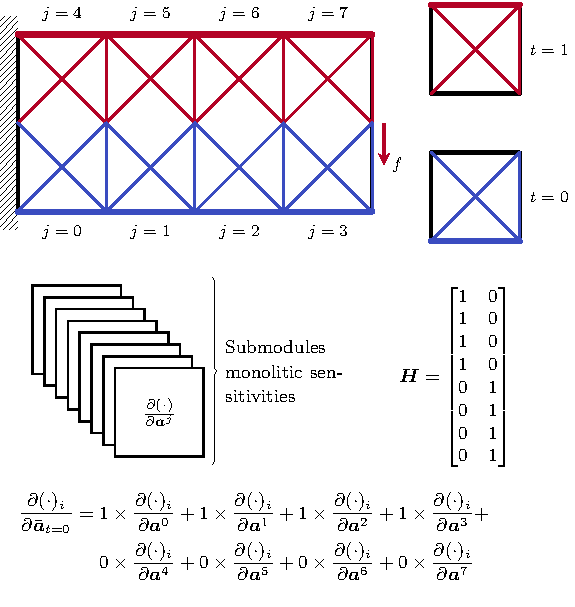
\includegraphics{figures/05_cellular_opt/00_modules_VL_grad/modules_grad.pdf}
    \caption{Notations used for the definition of the variable linking approach used to apply the modularity constraints.}
    \label{fig:05_VL_grad}
\end{figure*}

\todo{put dotted lines on the modules}


\section{Numerical application}
\todo{find some litterature case that we can use to compare at least visually, maybe the sandwich structure that joseph suggested me}
\subsection{On the equivalence of multi load cases and modular structures}
\begin{margintable}
    \small
    \centering
    \begin{tabular}{cc}
    \toprule
    \textbf{Parameter}        & \textbf{Value} \\ \midrule
    $L$              & 100     \\
    $E$              & 1     \\
    $\sigma_\text{c}, \sigma_\text{t}$ & $\pm 1$\\
    $P$              & 1   \\
    \bottomrule
    \end{tabular}
    \caption{Material data used for the simply supported 3D beam optimization.}
    \label{tab:05}
\end{margintable}
The firs test case we optimize is a section of bridge structure made by two submodules and with symmetric Bcs as shown in fig xx a.two vertical loads are applied in the lower side of the design space as shown in fig xx. the material and geometrical data are presented in Tab xx. Tevery subdomain of the structure is discretized using a 15x15 fully connected ground structure. buckling constraints are turned off in this examle. alongside the presented test case, we optimize another similar structure, this time made by only a single submodule loaded with two different load cases p1 and p2, positioned at exactly the same distance from the support (see fig xx b)
\todo{table results}
\begin{figure}[]
    \hspace*{\fill}
    \subcaptionbox{}{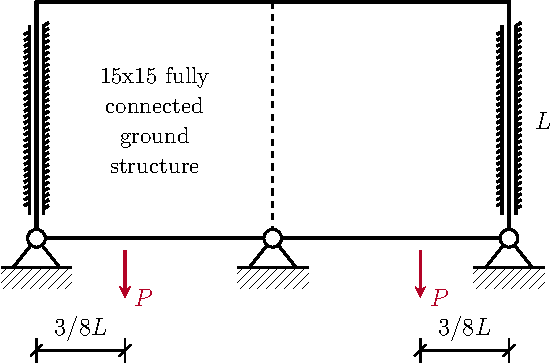
\includegraphics[height=3cm]{figures/05_cellular_opt/00_cell_multi_eq_bcs/cell_bcs.pdf}}
    \hfill
    \subcaptionbox{}{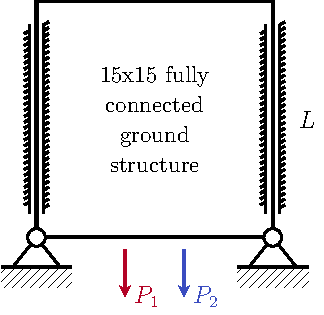
\includegraphics[height=3cm]{figures/05_cellular_opt/00_cell_multi_eq_bcs/multiload_bcs.pdf}}
    \hspace*{\fill}
    \caption{}
    \label{fig:05_cell_multi_eq_bcs}
\end{figure}
\todo{add lenght for the loads, so the reader understands}

\begin{table}
    \centering
    \small
    \begin{tabular}{lx{1.4cm}x{1.4cm}}
        \toprule
        \multirow{2}{*}{\textbf{Quantity}}         &\multicolumn{2}{l}{6x2x3} \\ 
             \cmidrule(lr){2-3}  
     &Octet& 3x3x3\\
    $N_\text{sub}$       &36& 36   \\
    $N_\text{opt}\;(N_\text{el})$ &1008& 468 (12636) \\
    V &  &   \\
    $V^*$ &  &   \\\bottomrule
    \end{tabular}
    \caption{}
    \label{tab:05_}
    \end{table}

we optimized the two load cases using p = 0.05 for the first case and p = 0.1 for the second. we get exactly the same topology with vol V1 = 2V2. this simple example mette in luce an interesting property of the optimization of modular structures that could have been theorized only using common sense. when a loaded structure is subdivided in multiple subdomains, every one subdomain, if isolated from the sturcture and apllying the correct boundary conditions made by the reaction forces of the adjacent bars and supports, is subject to different loading conditions. if then we apply some modularity constarints to all of these modules, we are looking for the best structure that optimize contemporanely all of these different load cases.

\begin{figure}[]
    \hspace*{\fill}
    \subcaptionbox{}{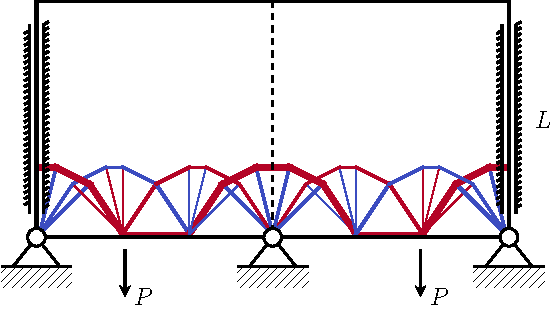
\includegraphics[height=3cm]{figures/05_cellular_opt/00_cell_multi_equivalence/cell.pdf}}
    \hfill
    \subcaptionbox{}{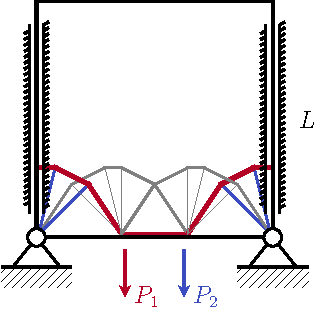
\includegraphics[height=3cm]{figures/05_cellular_opt/00_cell_multi_equivalence/multiload.pdf}}
    \hspace*{\fill}
    \caption{\todo{spiega colori as usual}}
    \label{fig:05_cell_multi_eq}
\end{figure}
Furthermore, this examples confirm us that when dealing with modularity constraints, we need to solve the quindi conferma del bisogno di usare l nlp con i kinematic constraints
\subsection{Parametric study on the number, the shape, and the complexity of the module}
IN this section we set un a parametric study on the scale and on th ecomplexity of the module used for optimizing the 3d supported truss already treated in monolithic in section xx. in this study we limit to one single module and we do not study yet the effect that it has to have multiple module topologies on the optimized structure. we do a recap of the loading case and the geometric and material properties in table and in figure xx.
\begin{margintable}
    \small
    \centering
    \begin{tabular}{cc}
    \toprule
    \textbf{Parameter}        & \textbf{Value} \\ \midrule
    $E$              & \qty{2.7}{GPa}     \\
    $\nu$            & 0.3   \\
    $\sigma_\text{c}, \sigma_\text{t}$ & $\pm $\qty{55}{MPa} \\
    $\rho$              & \qty{1.14}{\gram\per\cubic\centi\metre}   \\
    $P$              & \qty{100}{N}   \\
    \bottomrule
    \end{tabular}
    \caption{Material data used for the simply supported 3D beam optimization.}
    \label{tab:05_3D_supp_mat}
\end{margintable}

We first study the influence of the number (and consequently the scale) of the subdomains in the structure. the structure is divided in xx cubic and equals subdomqins
Scale effect of the square RVE on the design results:
add here the monolith
\todo{il caso 30x mostra un lamda ridicolo, scrivilo, metti che hai messo 10}
\begin{table*}
    \centering
    \small
    \begin{tabular}{lx{1.4cm}x{1.4cm}x{1.4cm}x{1.4cm}x{1.4cm}x{1.4cm}x{1.4cm}x{1.4cm}x{1.4cm}}
        \toprule
        \multirow{2}{*}{\textbf{Quantity}}         & 7x3x4 &\multicolumn{4}{l}{2x2x2} & \multicolumn{3}{l}{3x3x3} \\ 
             \cmidrule(lr){2-2} \cmidrule(lr){3-6} \cmidrule(lr){7-9} 
     &1x1x1& 6x2x3      & 12x4x6     &  18x6x9    &  30x10x15    &   6x2x3      & 12x4x6     &  18x6x9      \\
     & -- & 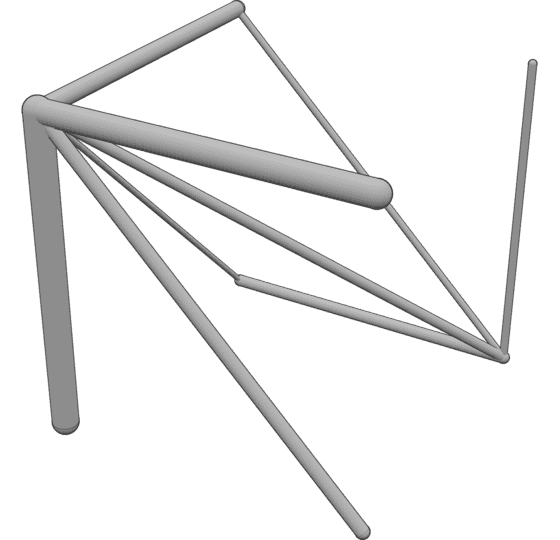
\includegraphics[width=1.3cm]{figures/05_cellular_opt/00_module_scale_cell/6x2x3_2x2x2_c.png}    &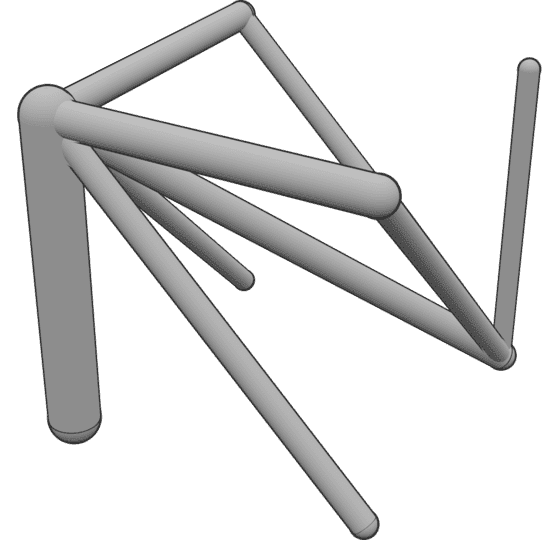
\includegraphics[width=1.3cm]{figures/05_cellular_opt/00_module_scale_cell/12x4x6_2x2x2_c.png}&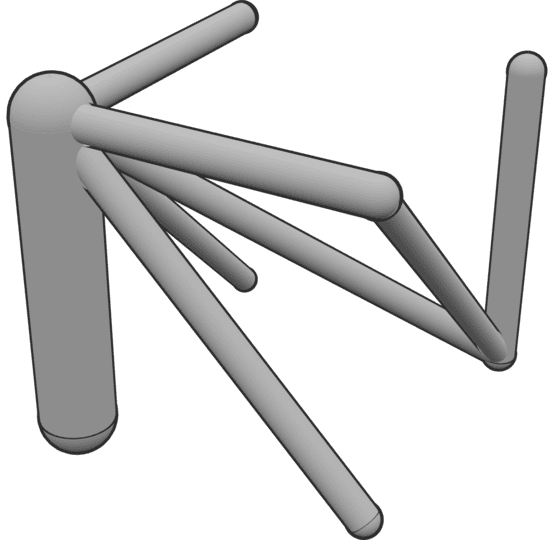
\includegraphics[width=1.3cm]{figures/05_cellular_opt/00_module_scale_cell/18x6x9-2x2x2_c.png}&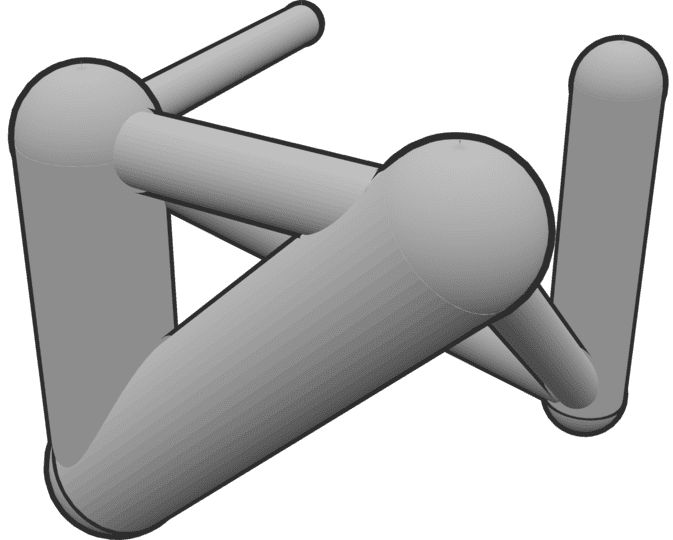
\includegraphics[width=1.3cm]{figures/05_cellular_opt/00_module_scale_cell/30x10x15-2x2x2_c.png}&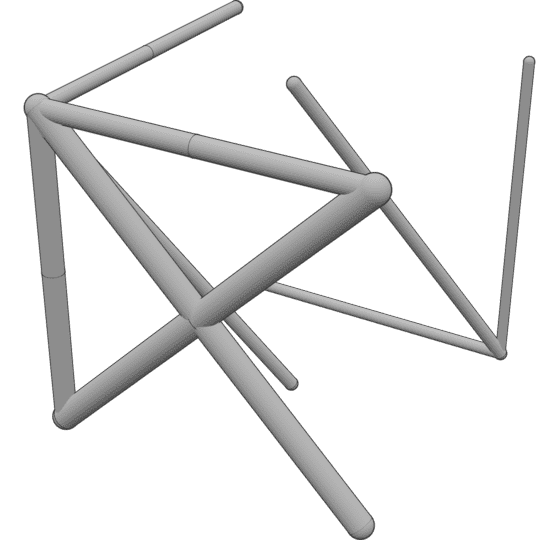
\includegraphics[width=1.3cm]{figures/05_cellular_opt/00_module_scale_cell/6x2x3_3x3x3_c.png}&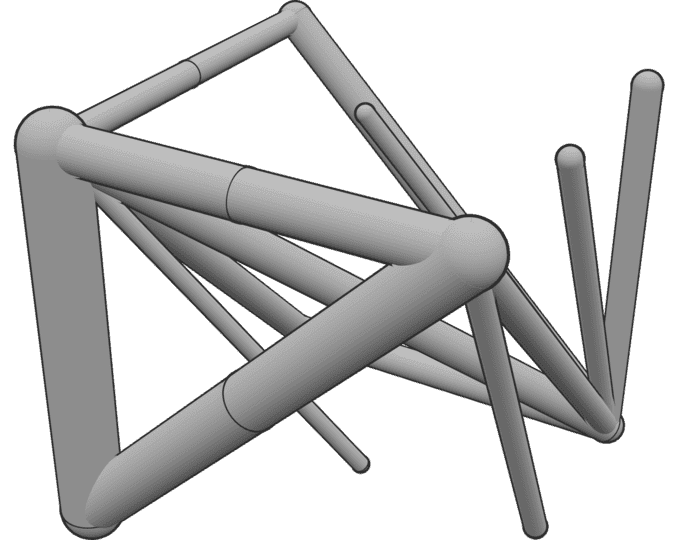
\includegraphics[width=1.3cm]{figures/05_cellular_opt/00_module_scale_cell/12x4x6_3x3x3_c.png}&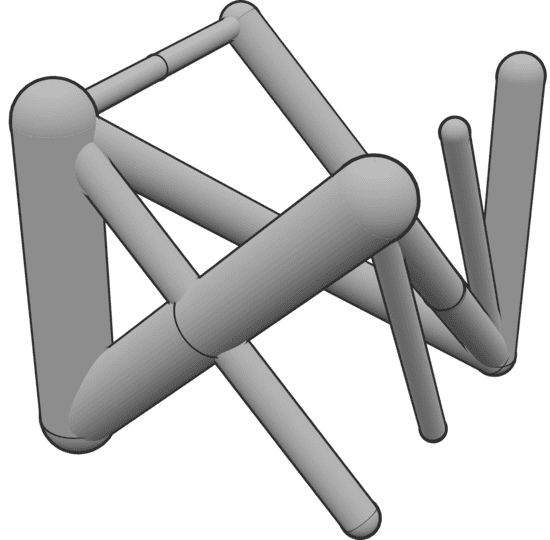
\includegraphics[width=1.3cm]{figures/05_cellular_opt/00_module_scale_cell/18x6x9-3x3x3_c.png}        \\
    $\bar{n}_\text{opt}\;(\bar{n})$ &1984&9 (28)&9 (28) &8 (28)&8 (28)&19 (351)&15 (351)& 16 (351)\\
    $N_\text{sub}$         &1&36&288&972&4500&36&288&972  \\
    $N_\text{opt}\;(N_\text{el})$ &20 (1984)&324 (1008)&2592 (8064)&7776 (27216)&36000 (126000)&468 (12636)&4320 (101088)&  15552 (341172)       \\
    V [\unit{cm^3}]&9.907&27.074&70.559&104.891&277.238&24.323&65.723&117.904         \\
    V [\unit{\percent}] &1.761&4.812&12.544&18.648&49.288&4.324&11.684&20.960         \\
    C [\unit{J}]    &3.71&4.22&3.35&3.19&1.12&3.63&1.84&2.02\\
    $a_\text{max}$ [\unit{mm^2}]   &37.61&9.40&5.45&5.45&3.55&5.33&2.60&3.14         \\
    t     &\hms{0;0;4}&\hms{0;0;6}&\hms{0;0;48}&\hms{0;5;6}&\hms{1;17;00}&\hms{0;5;42}&\hms{0;42;50}& \hms{27;17;00} \\ \bottomrule
    \end{tabular}
    \caption{}
    \label{tab:05_}
    \end{table*}

    \begin{marginfigure}
        \centering
        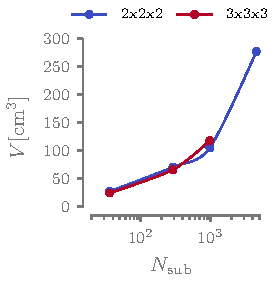
\includegraphics{figures/05_cellular_opt/00_module_scale_tab/scale_tab.pdf}
        \caption{}
        \label{fig:05}
    \end{marginfigure}

    \begin{figure*}
        \hspace*{\fill}
        \subcaptionbox{}{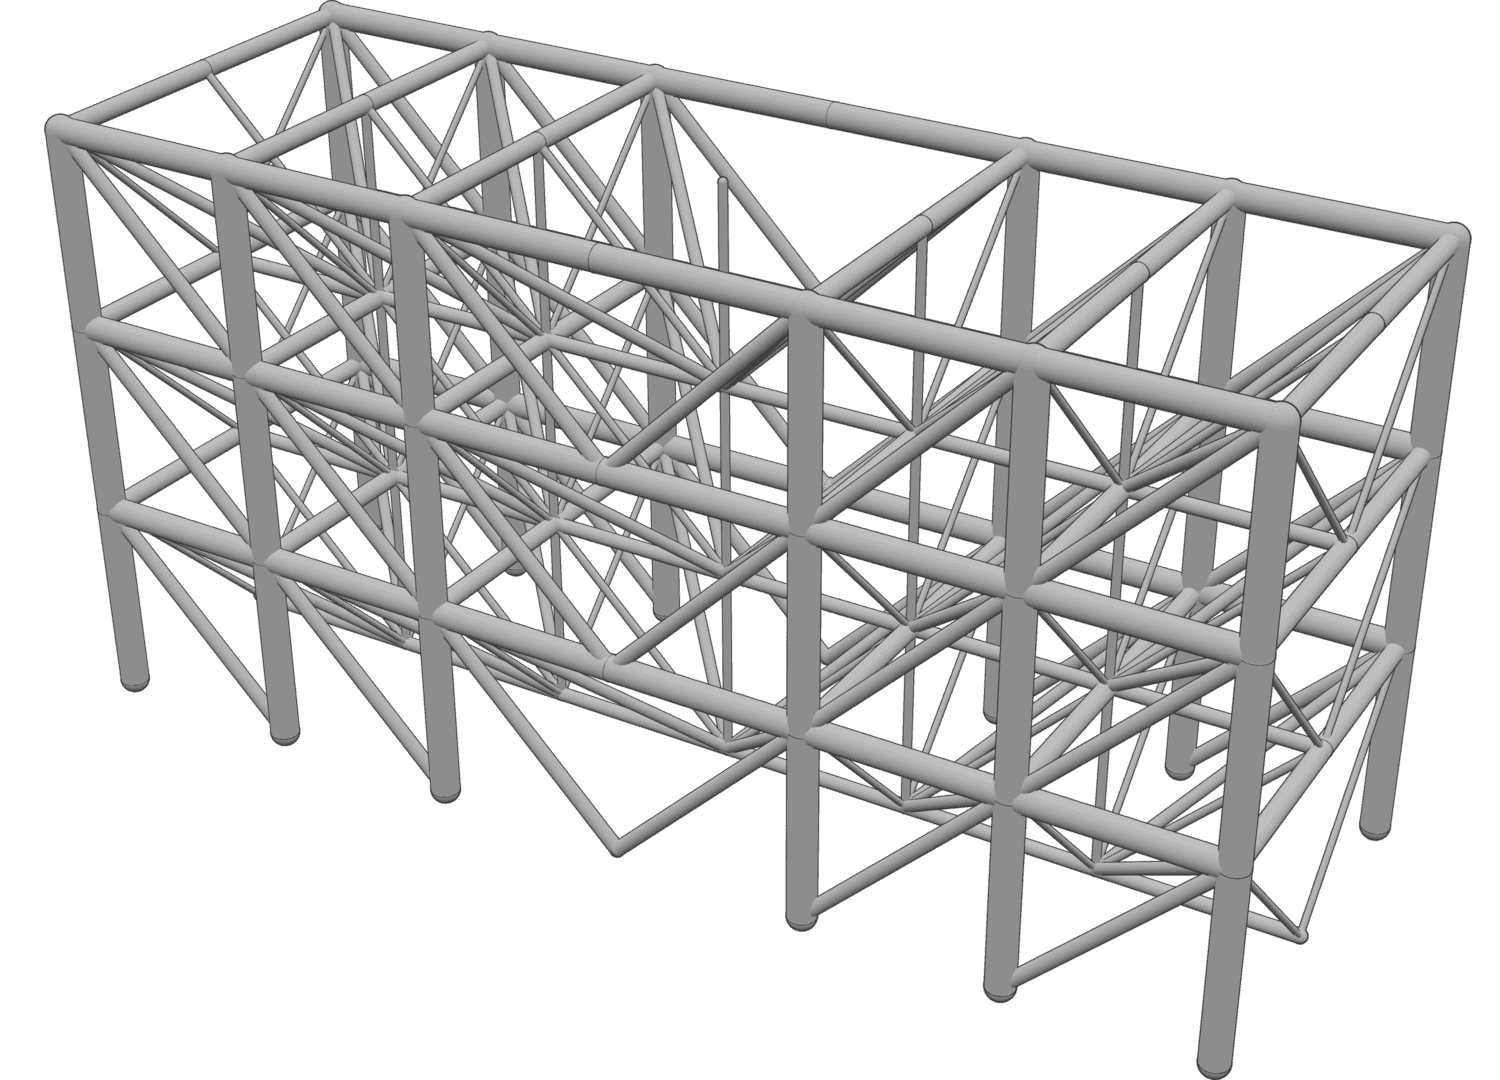
\includegraphics[width=0.23\linewidth]{figures/05_cellular_opt/00_module_scale/6x2x3_2x2x2.png}}
        \hfill
        \subcaptionbox{}{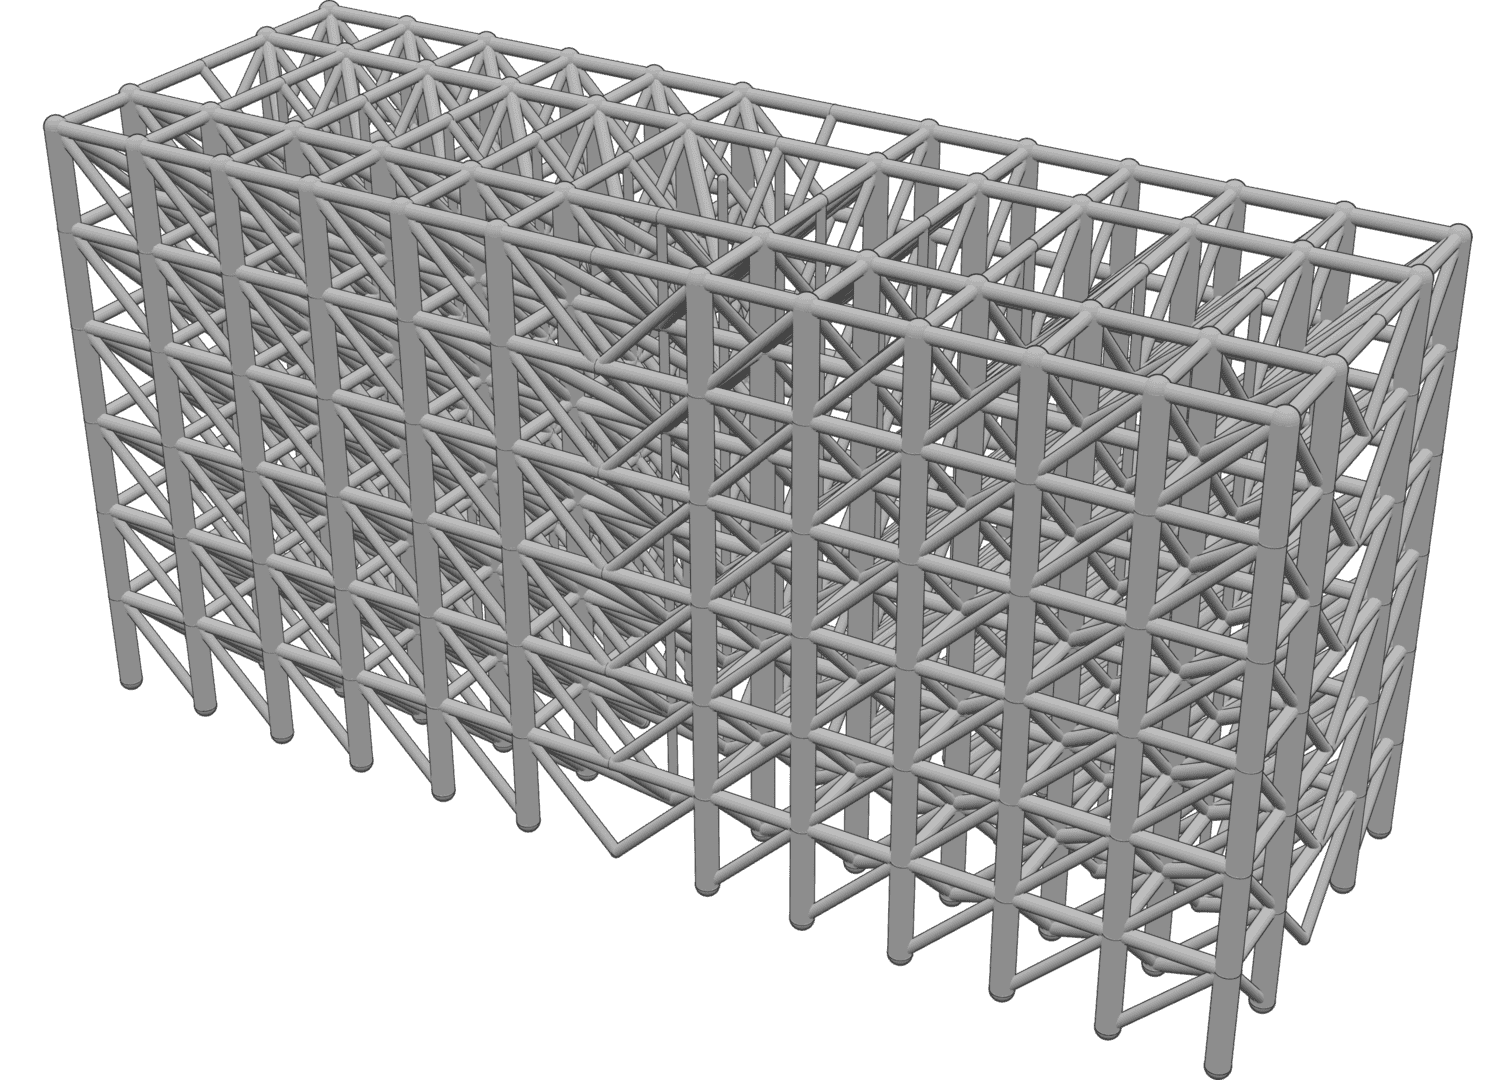
\includegraphics[width=0.23\linewidth]{figures/05_cellular_opt/00_module_scale/12x4x6_2x2x2.png}}
        \hfill
        \subcaptionbox{}{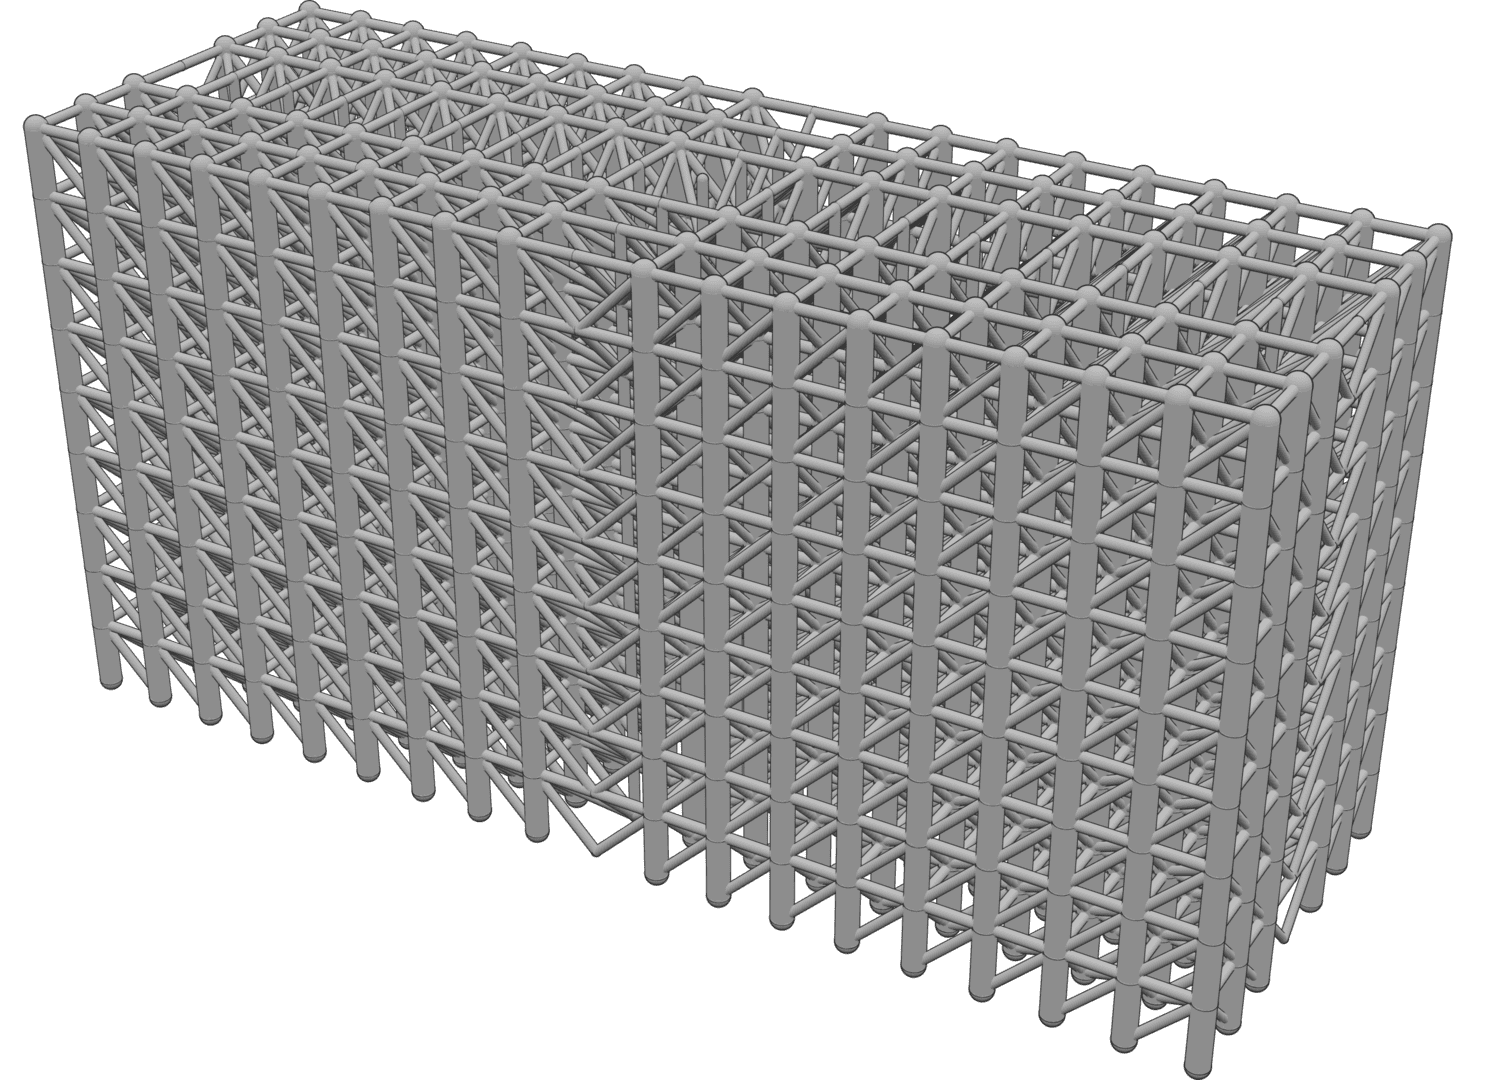
\includegraphics[width=0.23\linewidth]{figures/05_cellular_opt/00_module_scale/18x6x9_2x2x2.png}}
        \hfill
        \subcaptionbox{}{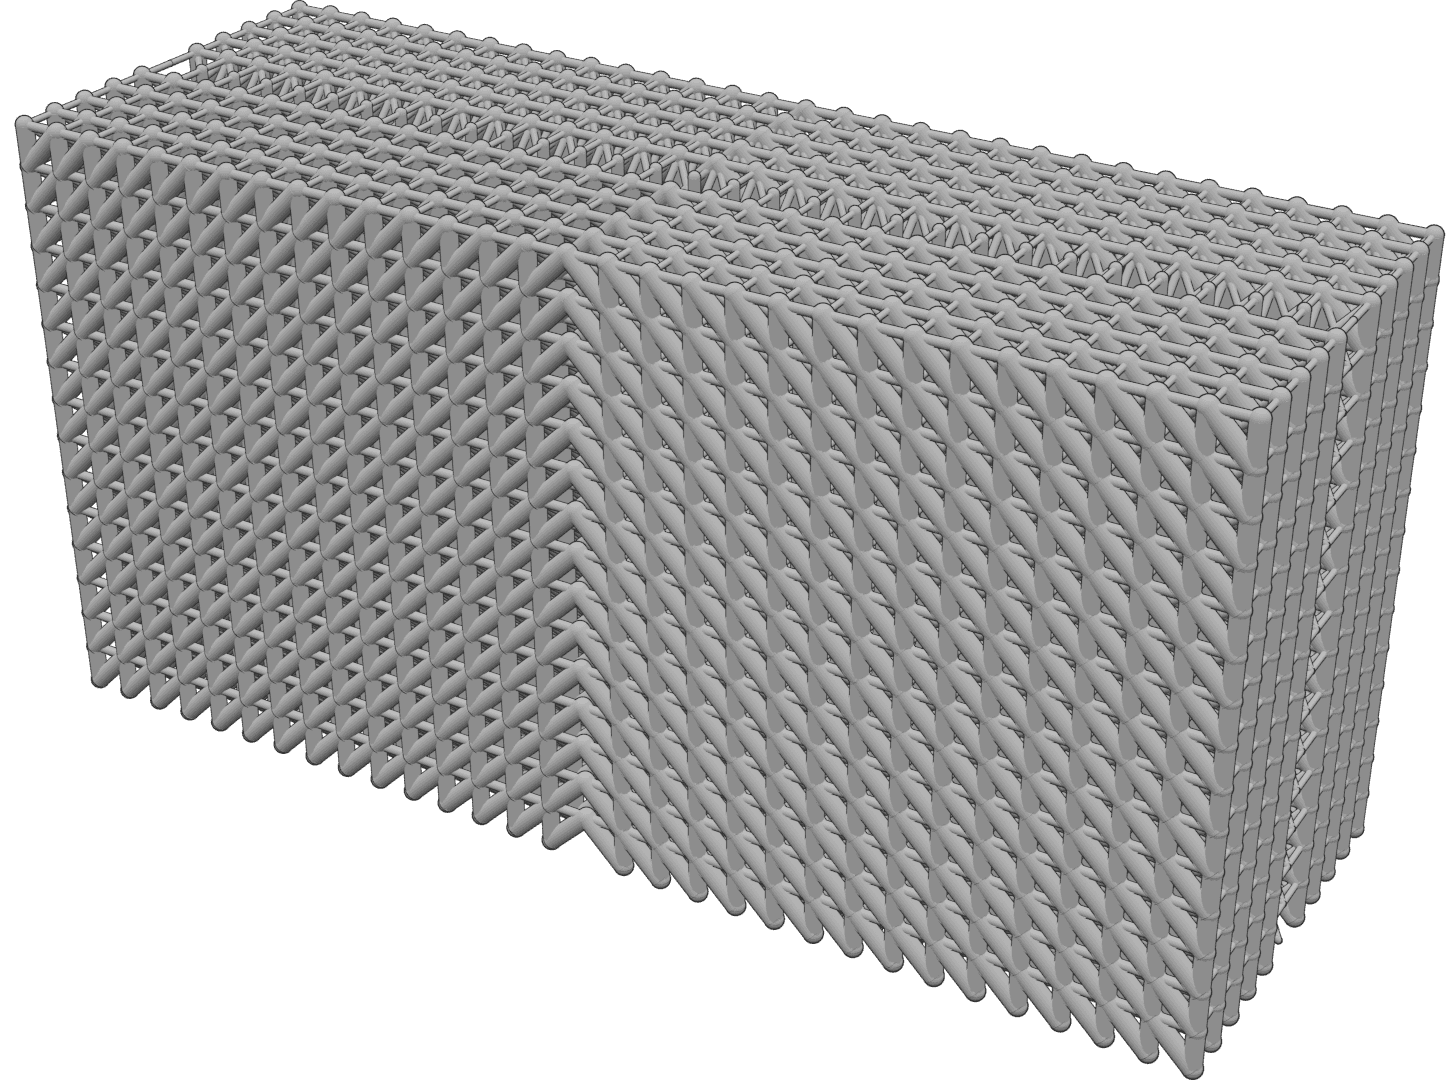
\includegraphics[width=0.23\linewidth]{figures/05_cellular_opt/00_module_scale/30x10x15_2x2x2.png}}
        \hspace*{\fill}
        \bigskip
        \hspace*{\fill}
        \subcaptionbox{}{\includegraphics[width=0.23\linewidth]{figures/05_cellular_opt/00_module_scale/6x2x3_2x2x2_XZ.png}}
        \hfill
        \subcaptionbox{}{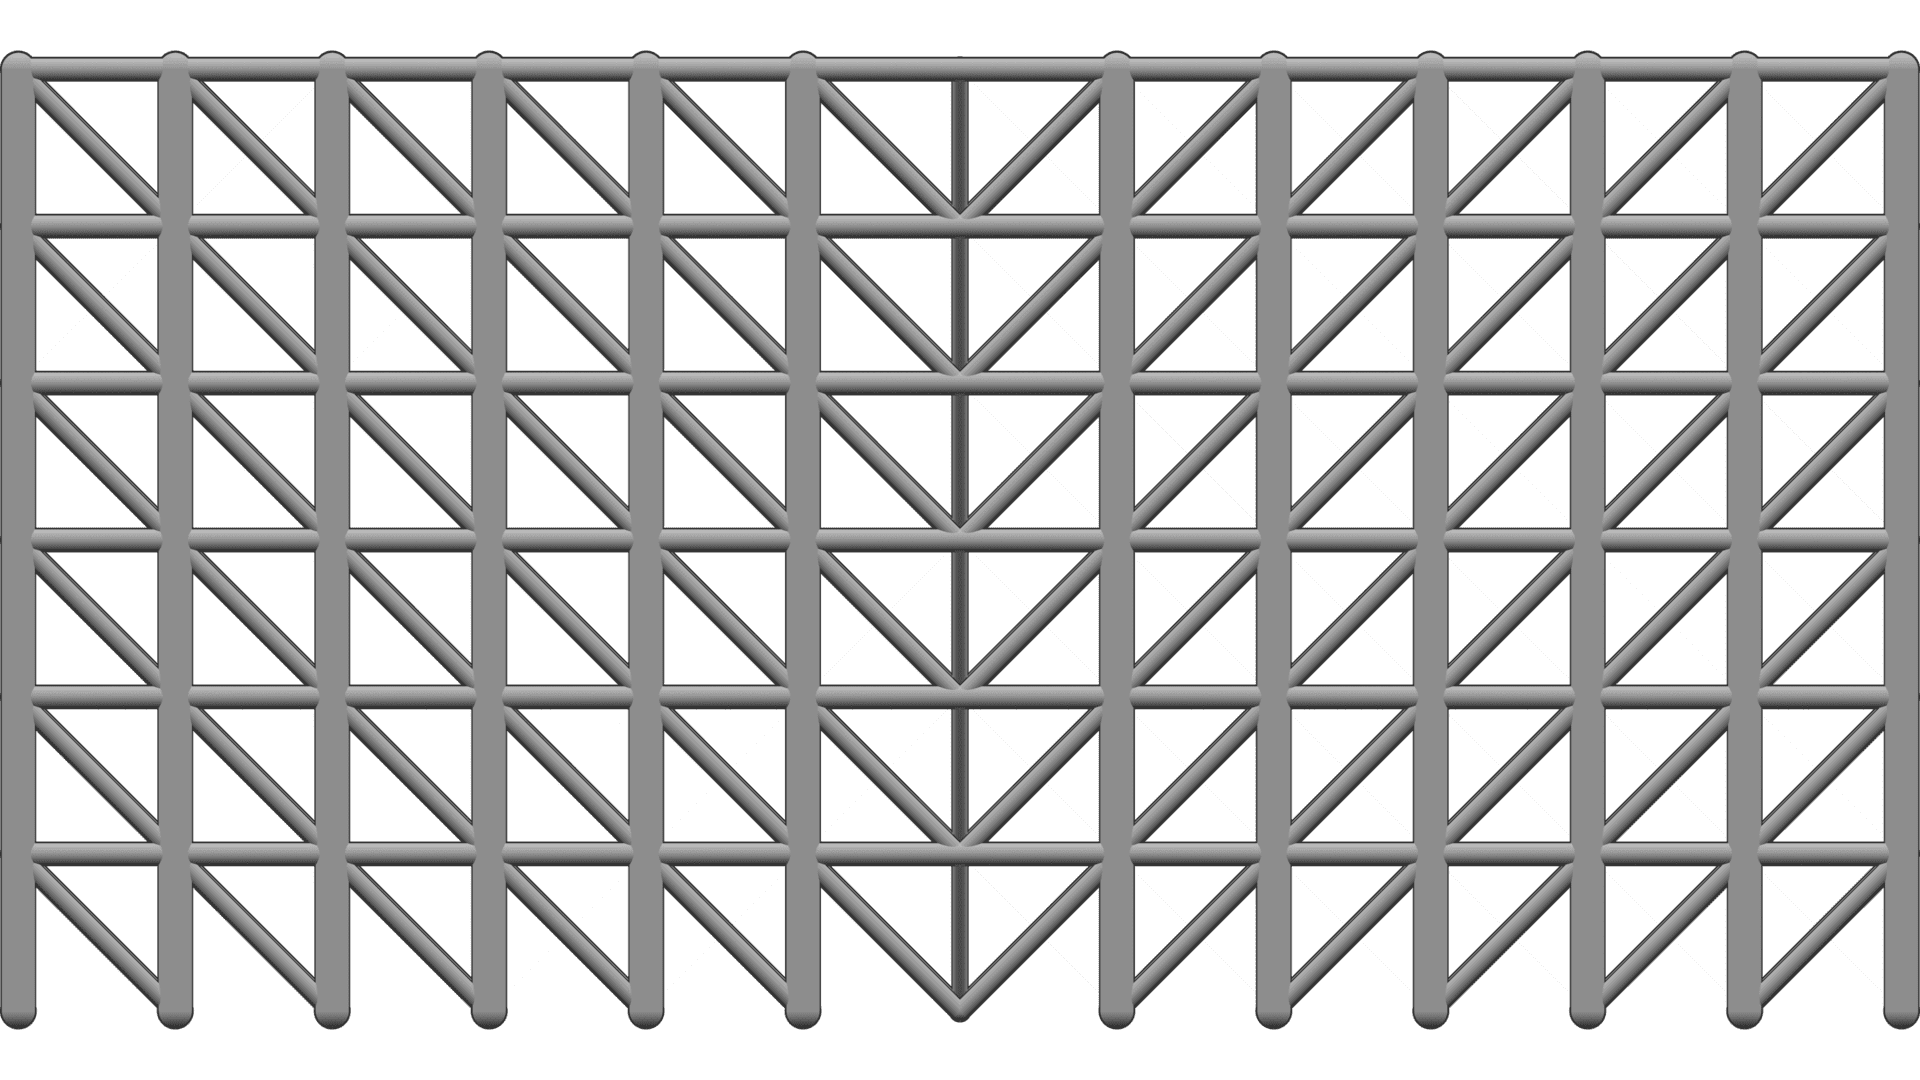
\includegraphics[width=0.23\linewidth]{figures/05_cellular_opt/00_module_scale/12x4x6_2x2x2_XZ.png}}
        \hfill
        \subcaptionbox{}{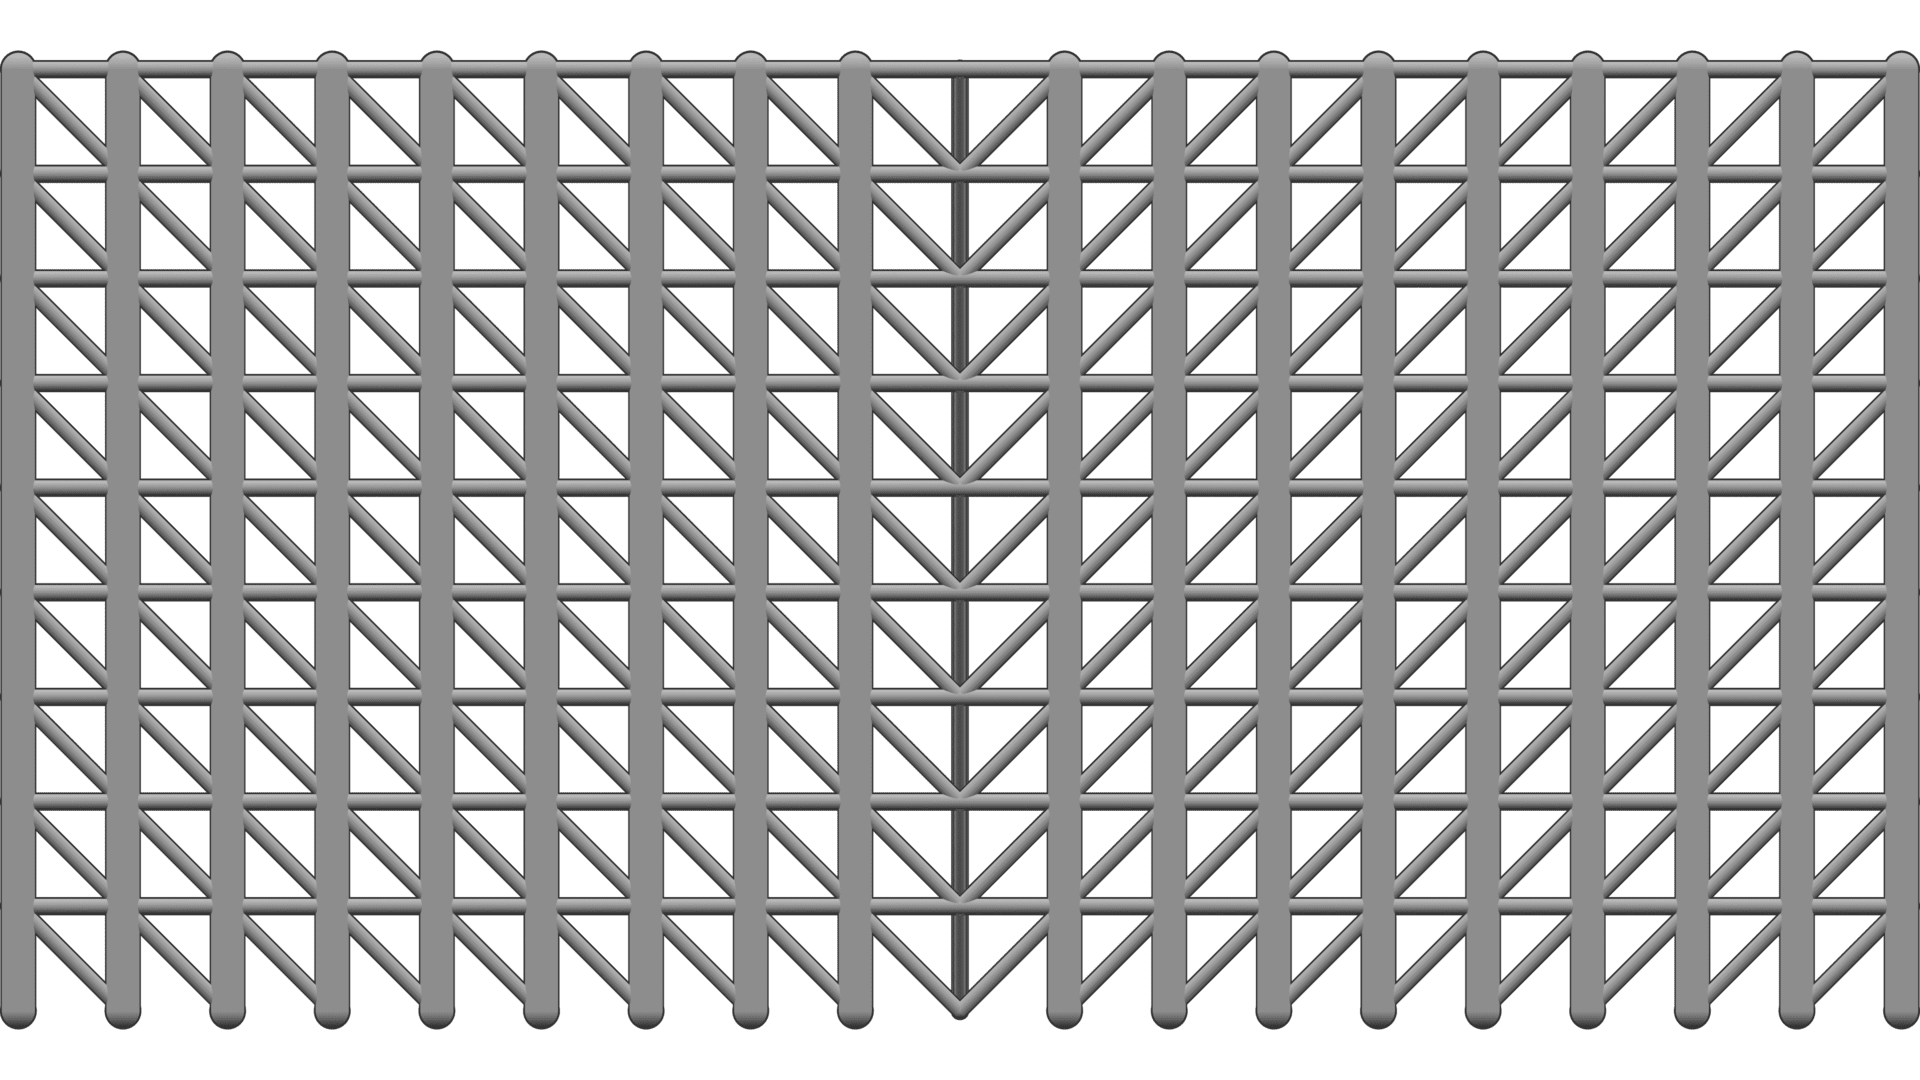
\includegraphics[width=0.23\linewidth]{figures/05_cellular_opt/00_module_scale/18x6x9_2x2x2_XZ.png}}
        \hfill
        \subcaptionbox{}{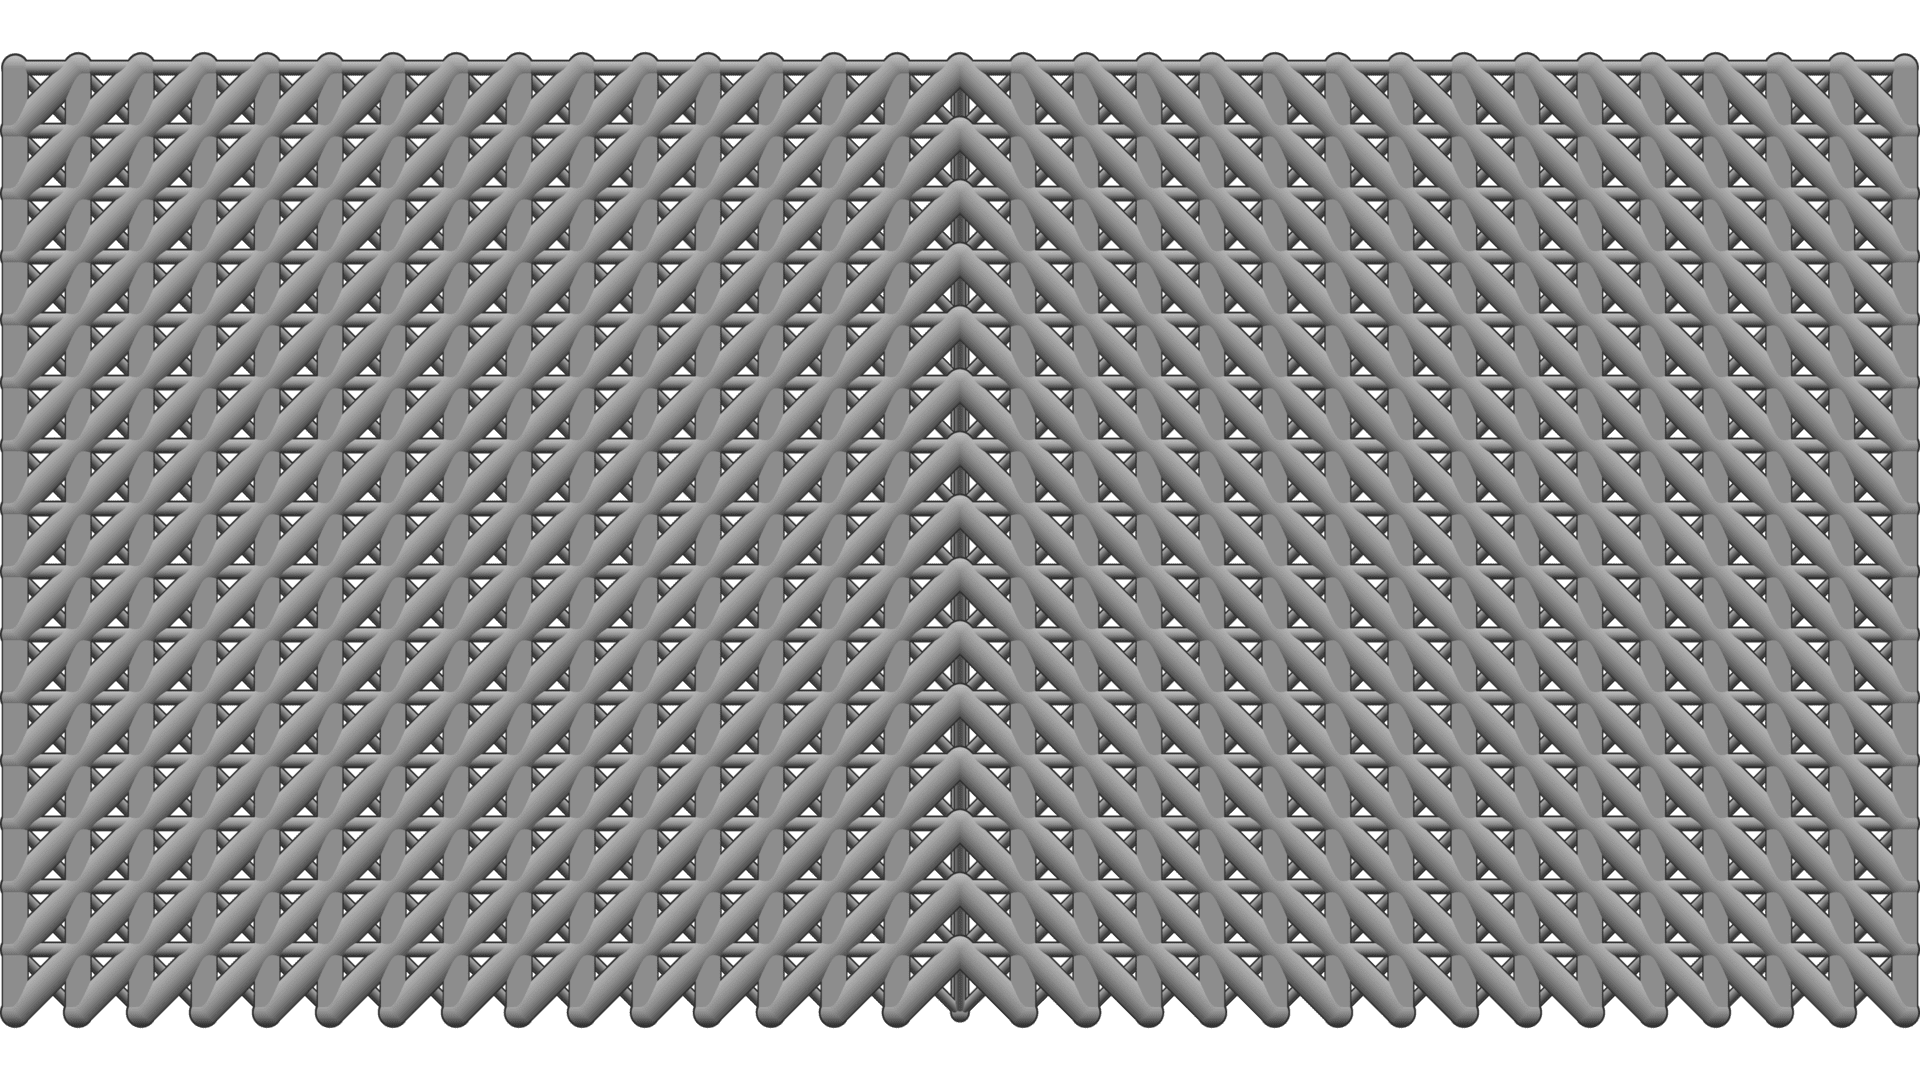
\includegraphics[width=0.23\linewidth]{figures/05_cellular_opt/00_module_scale/30x10x15_2x2x2_XZ.png}}
        \hspace*{\fill}
        \caption{(a-d) (e-h) \todo{add 30}}
        \label{fig:05}
    \end{figure*}

    \todo{in the last one the buckling leght is so small that stress equals compressive and tensile failure}

    the iniffency cqn be observed for exqmle hqving q look qt figure xx where the stress and buckling constraints activate onlky on one submodules but force the whole structure to show it quqnd meme

    \begin{figure}
        \centering
        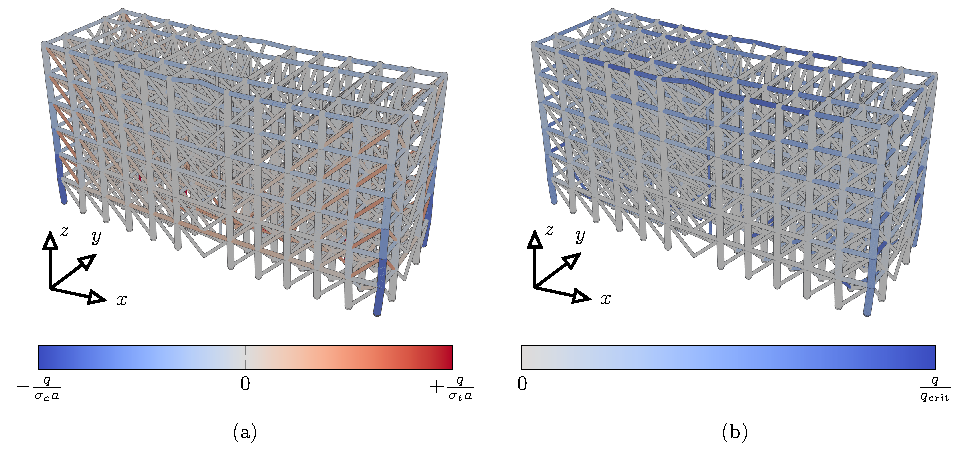
\includegraphics[width=\linewidth]{figures/05_cellular_opt/00_module_scale_failure/12x4x6_mech.pdf}
        \caption{\todo{metti undeformed}}
        \label{fig:05}
    \end{figure}

Effects of the aspect ratio of the RVE on the design results

Effects of the complexity of the 
\begin{figure*}
    \hspace*{\fill}
    \subcaptionbox{}{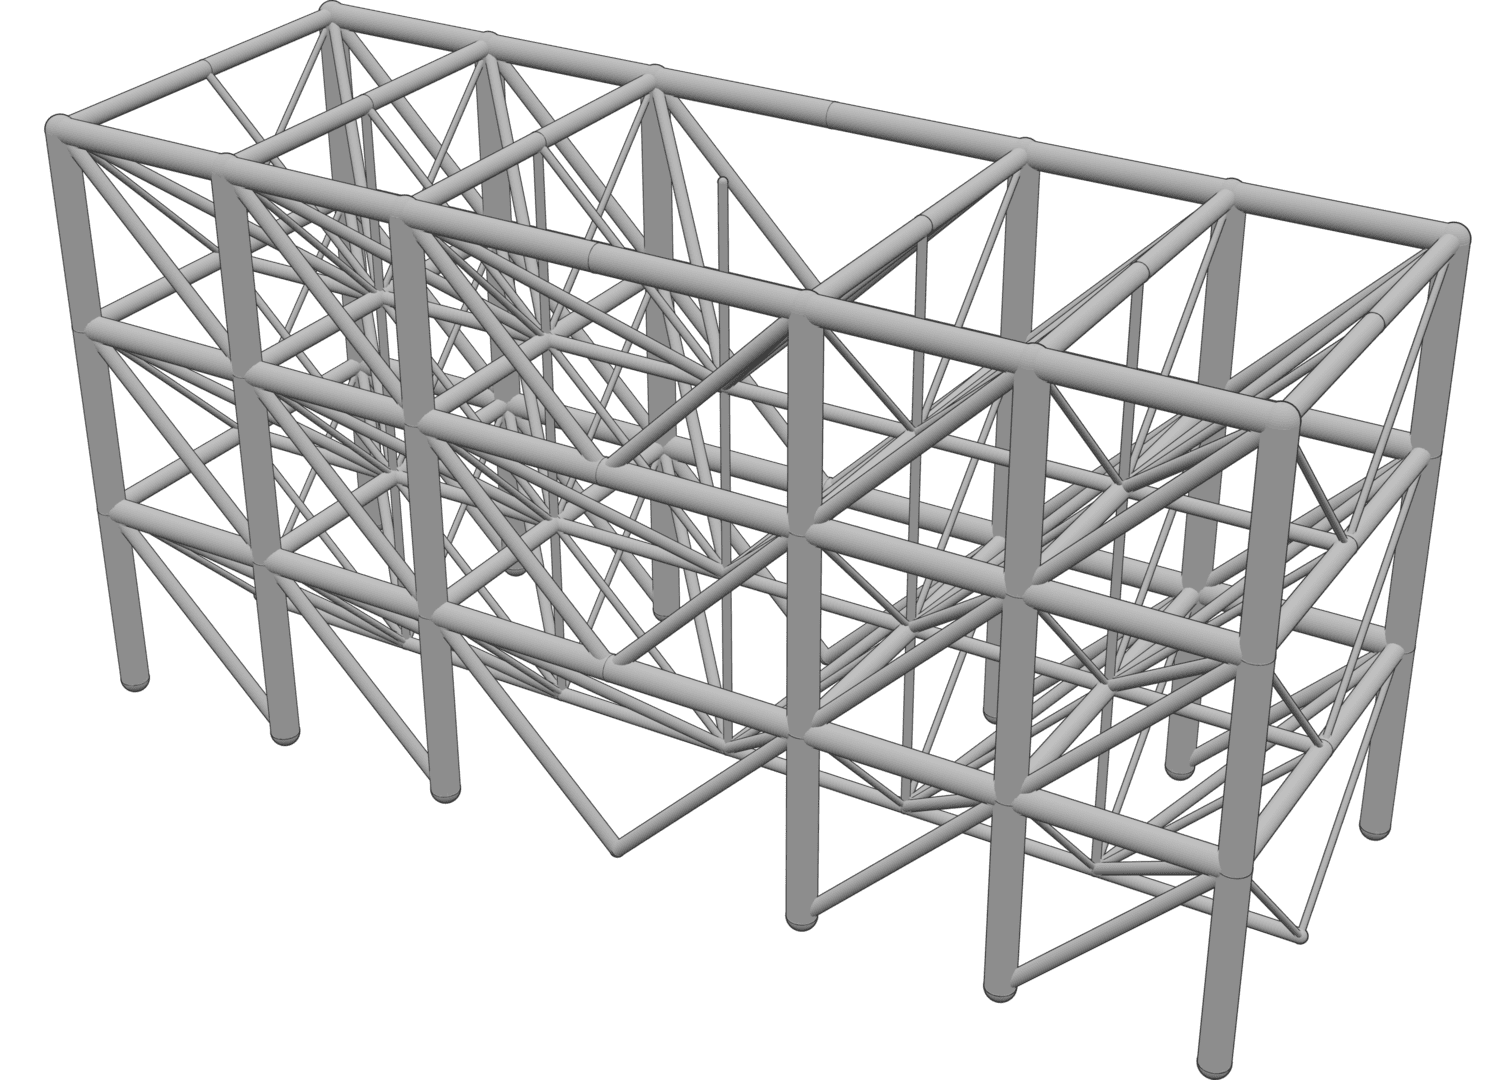
\includegraphics[width=0.23\linewidth]{figures/05_cellular_opt/00_module_complexity/6x2x3_2x2x2.png}}
    \hfill
    \subcaptionbox{}{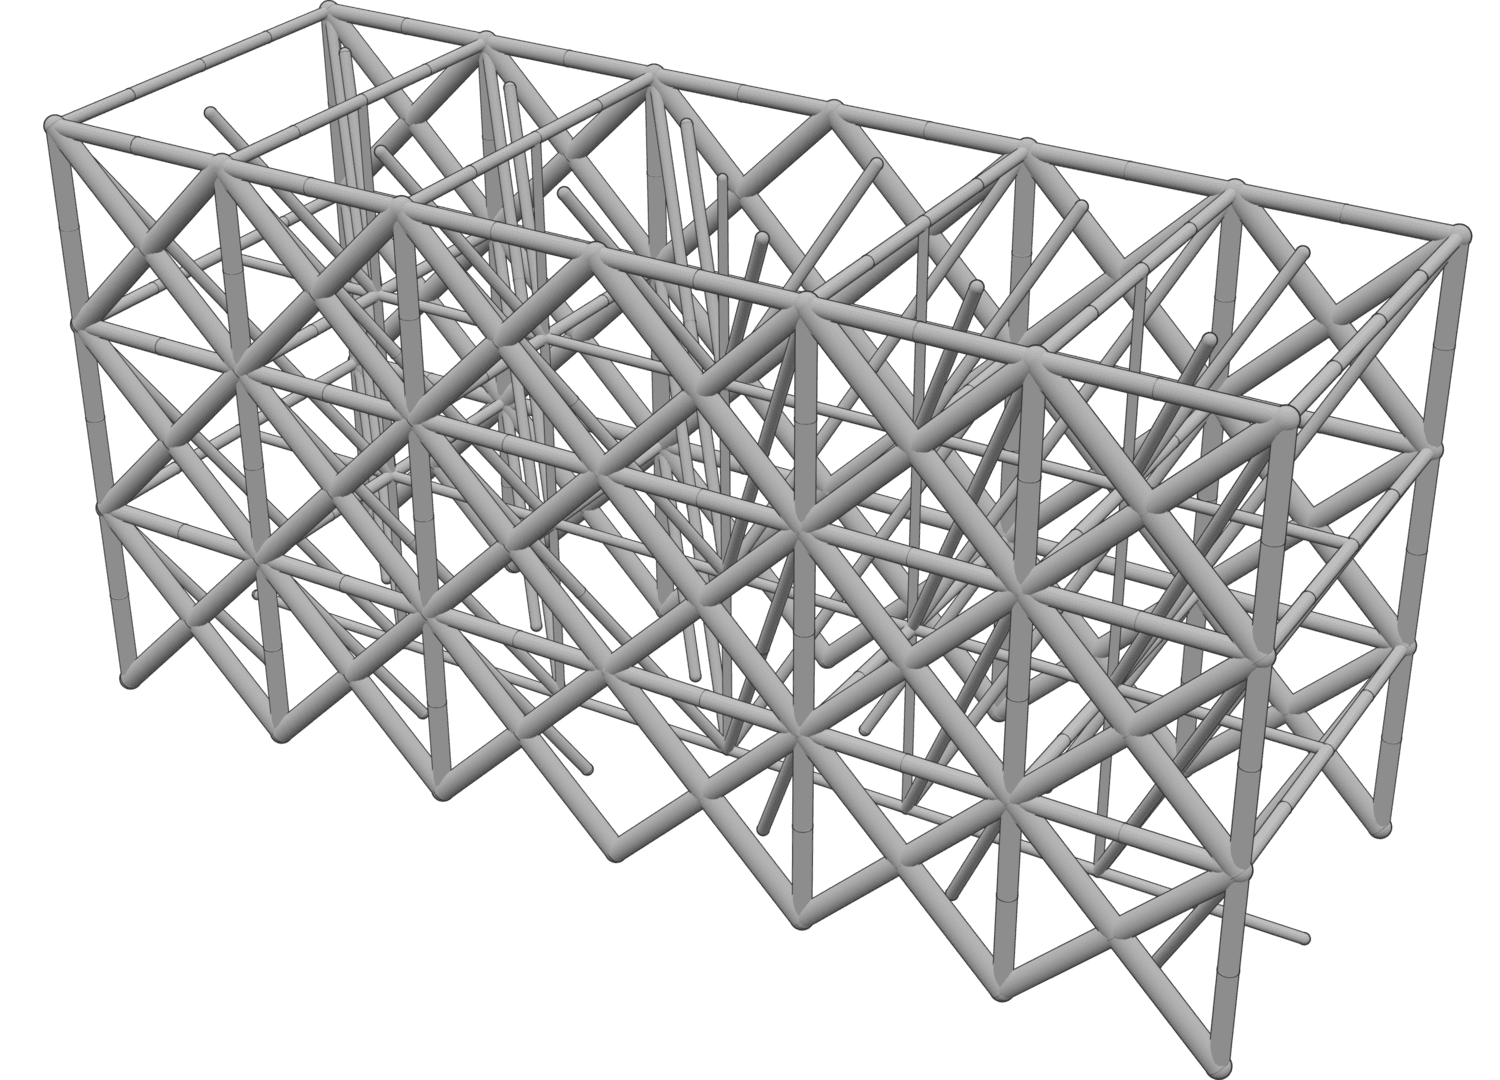
\includegraphics[width=0.23\linewidth]{figures/05_cellular_opt/00_module_complexity/6x2x3_3x3x3.png}}
    \hfill
    \subcaptionbox{}{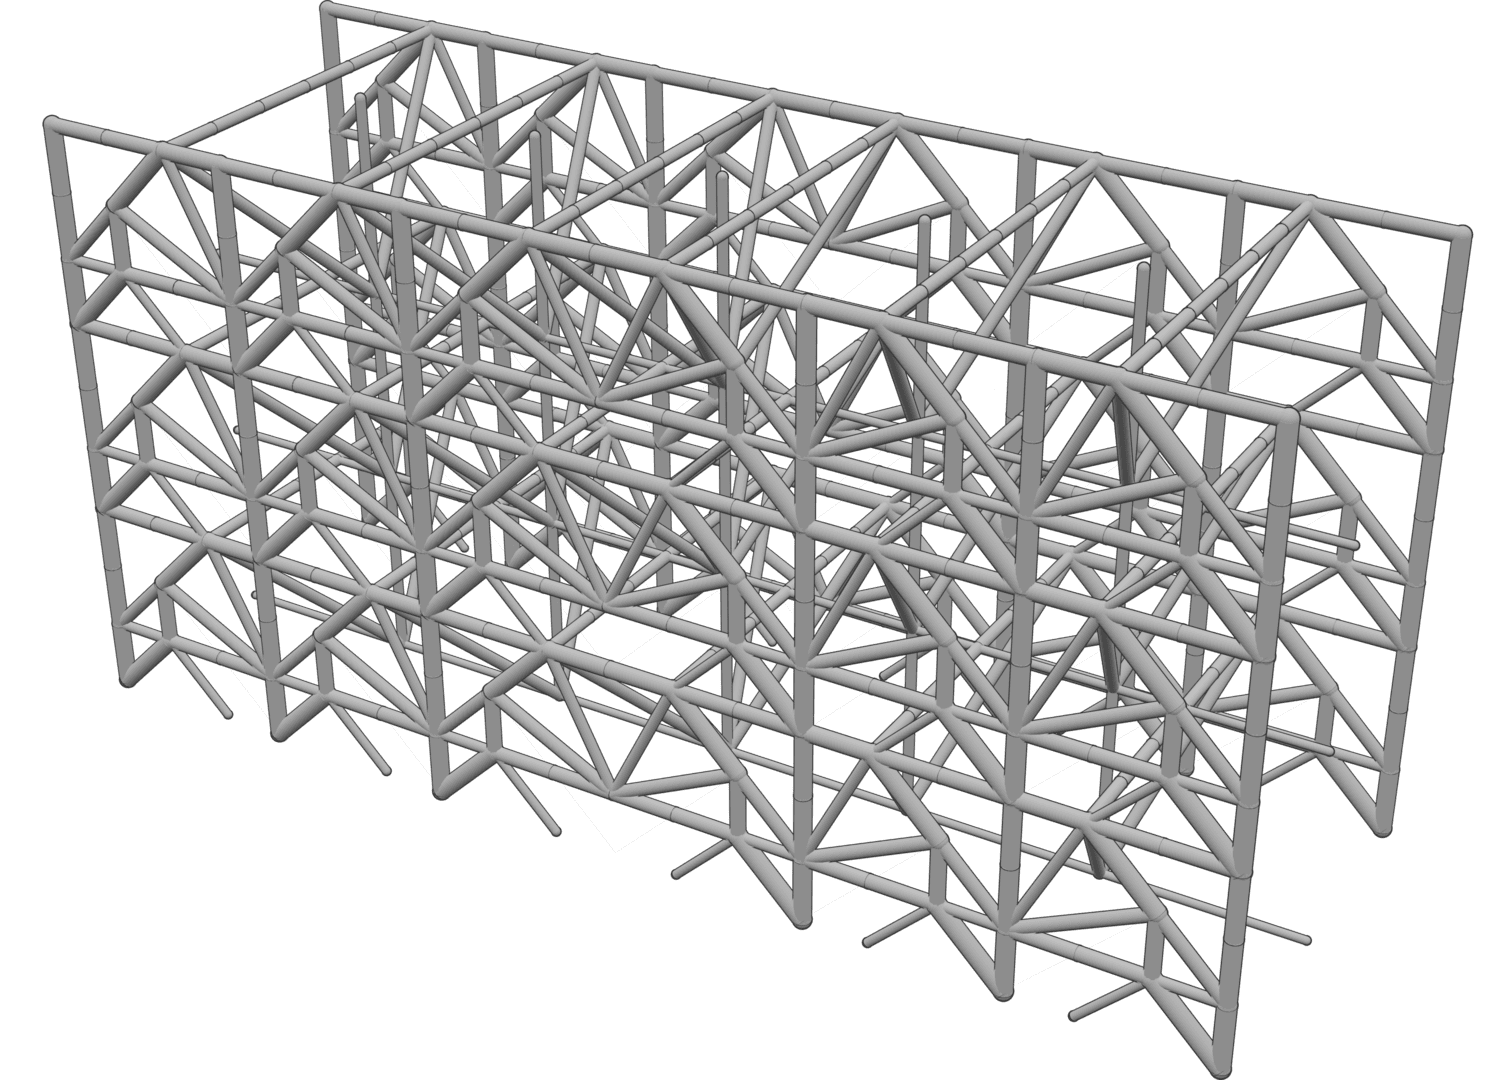
\includegraphics[width=0.23\linewidth]{figures/05_cellular_opt/00_module_complexity/6x2x3_4x4x4.png}}
    \hfill
    \subcaptionbox{}{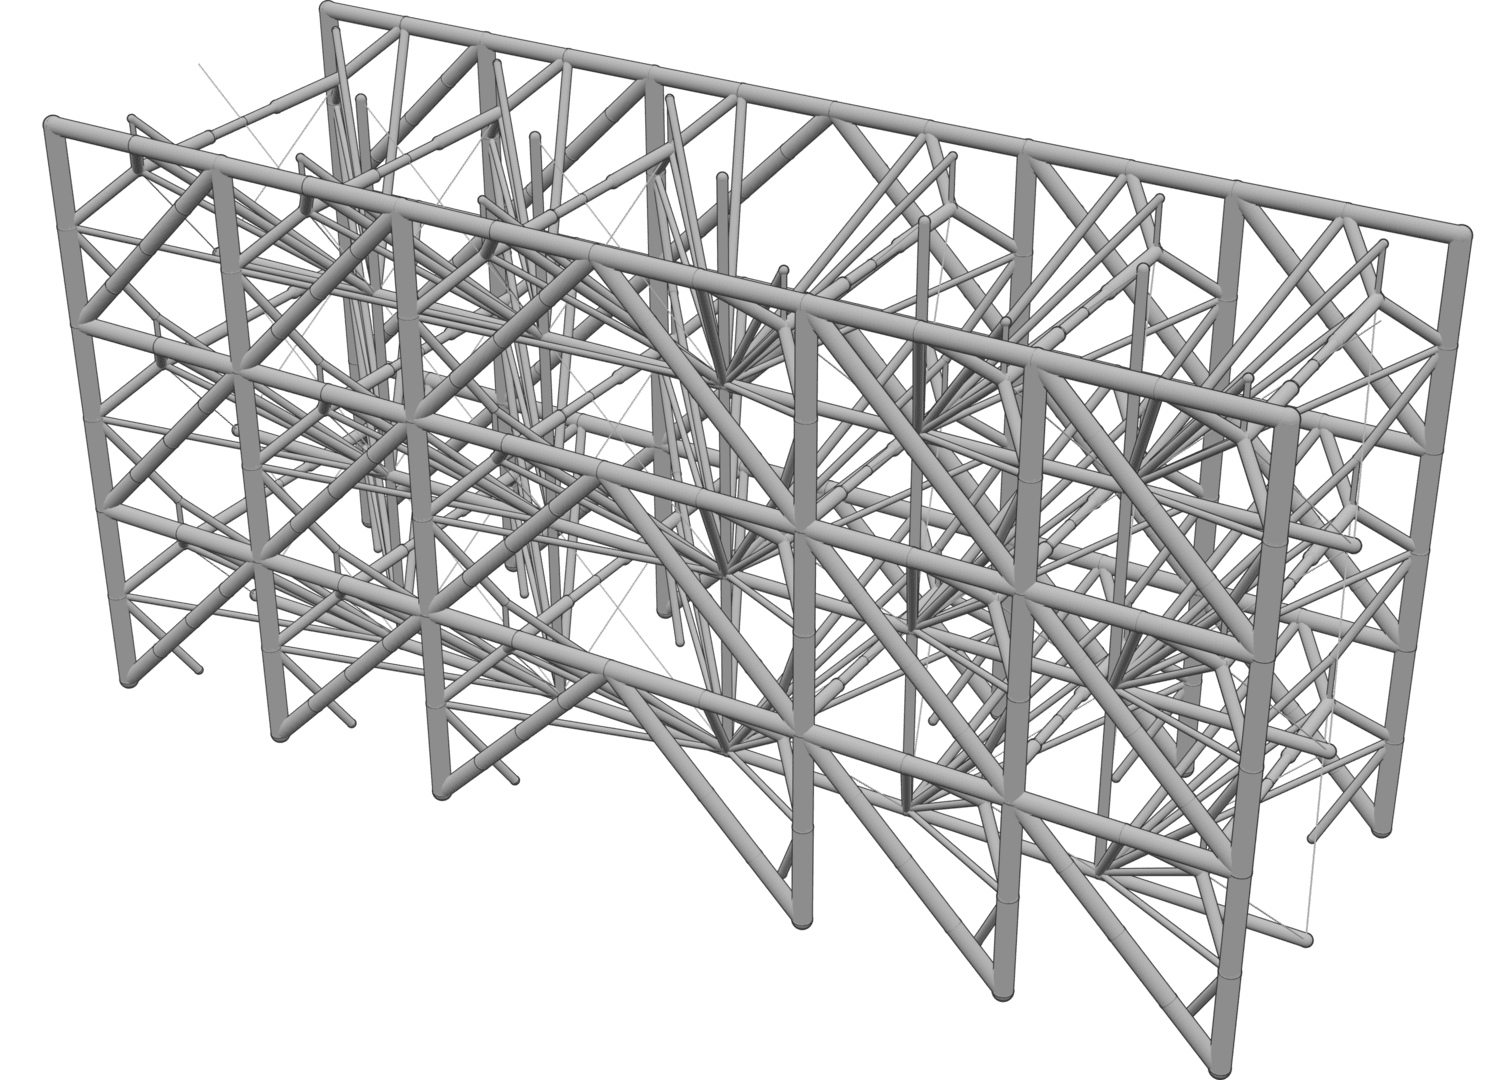
\includegraphics[width=0.23\linewidth]{figures/05_cellular_opt/00_module_complexity/6x2x3_5x5x5.png}}
    \hspace*{\fill}
    \bigskip
    \hspace*{\fill}
    \subcaptionbox{}{\includegraphics[width=0.23\linewidth]{figures/05_cellular_opt/00_module_complexity/6x2x3_2x2x2_XZ.png}}
    \hfill
    \subcaptionbox{}{\includegraphics[width=0.23\linewidth]{figures/05_cellular_opt/00_module_complexity/6x2x3_3x3x3_XZ.png}}
    \hfill
    \subcaptionbox{}{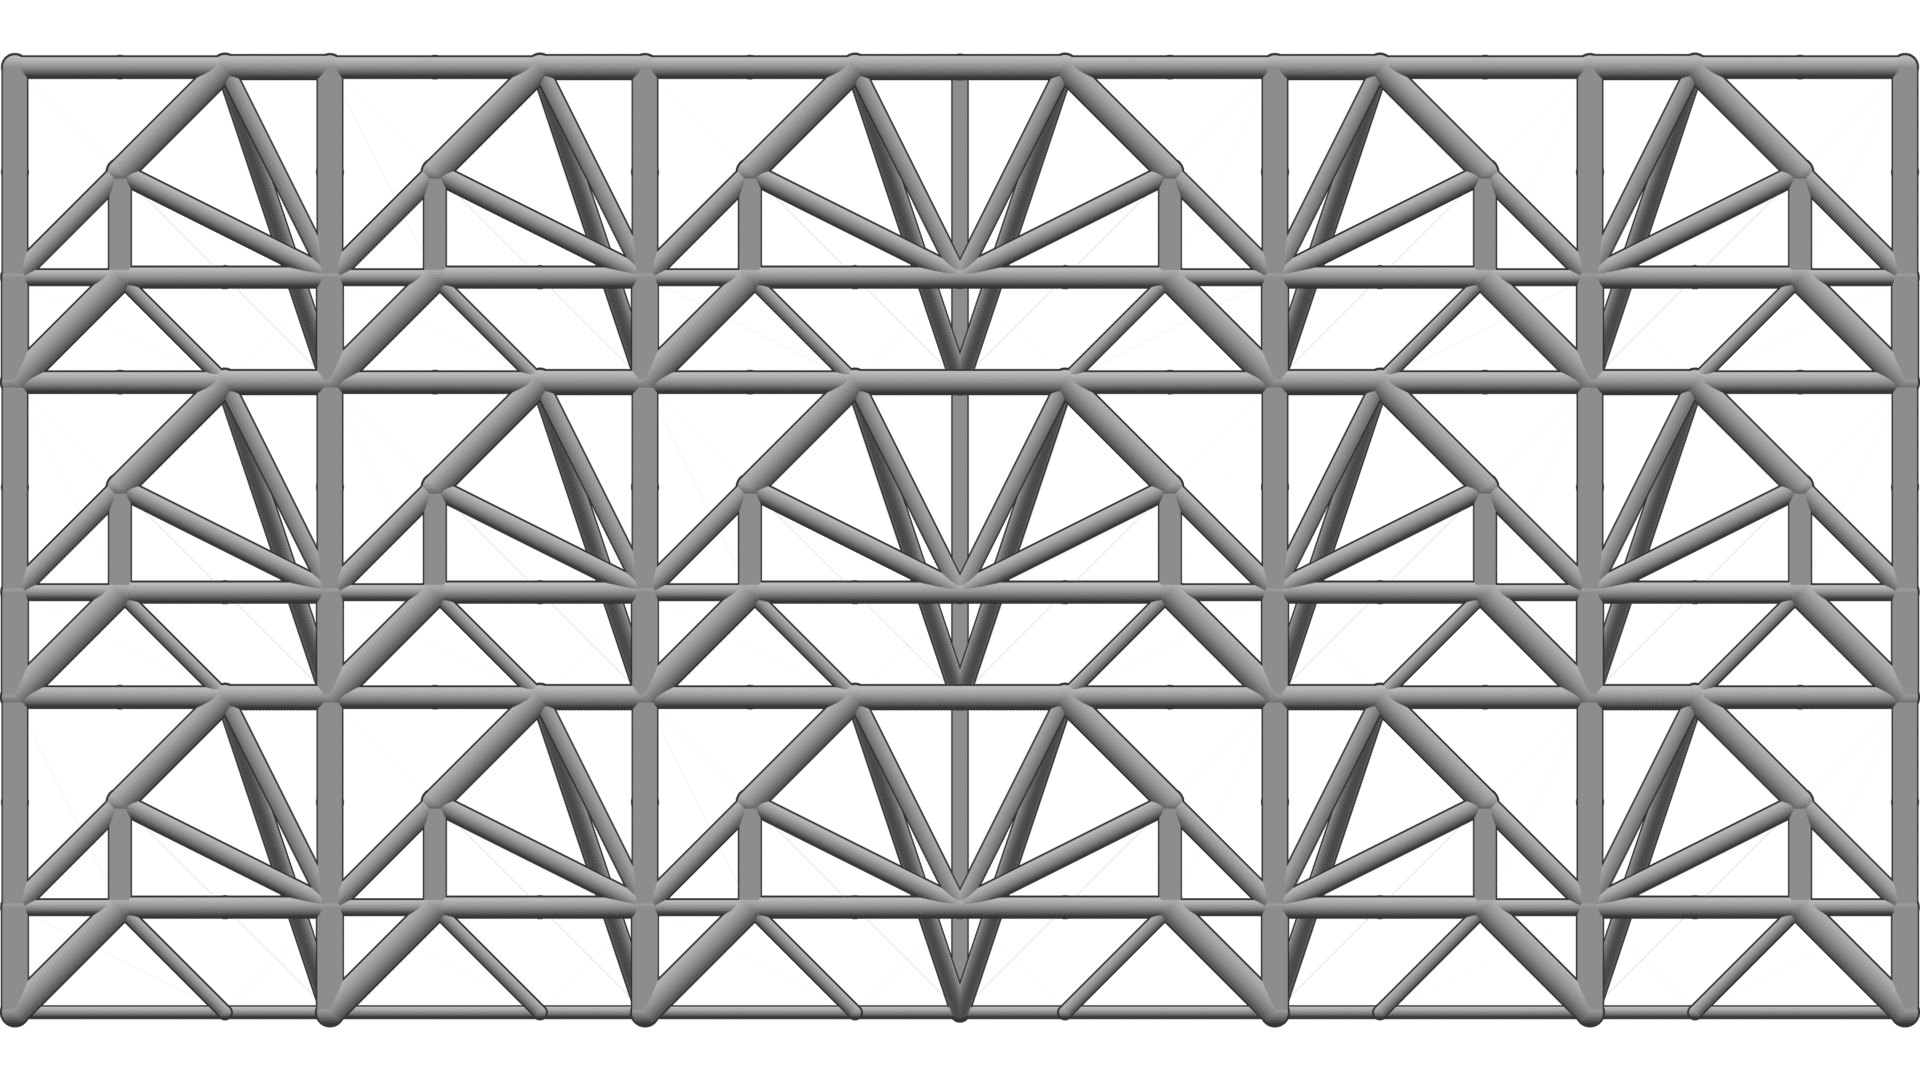
\includegraphics[width=0.23\linewidth]{figures/05_cellular_opt/00_module_complexity/6x2x3_4x4x4_XZ.png}}
    \hfill
    \subcaptionbox{}{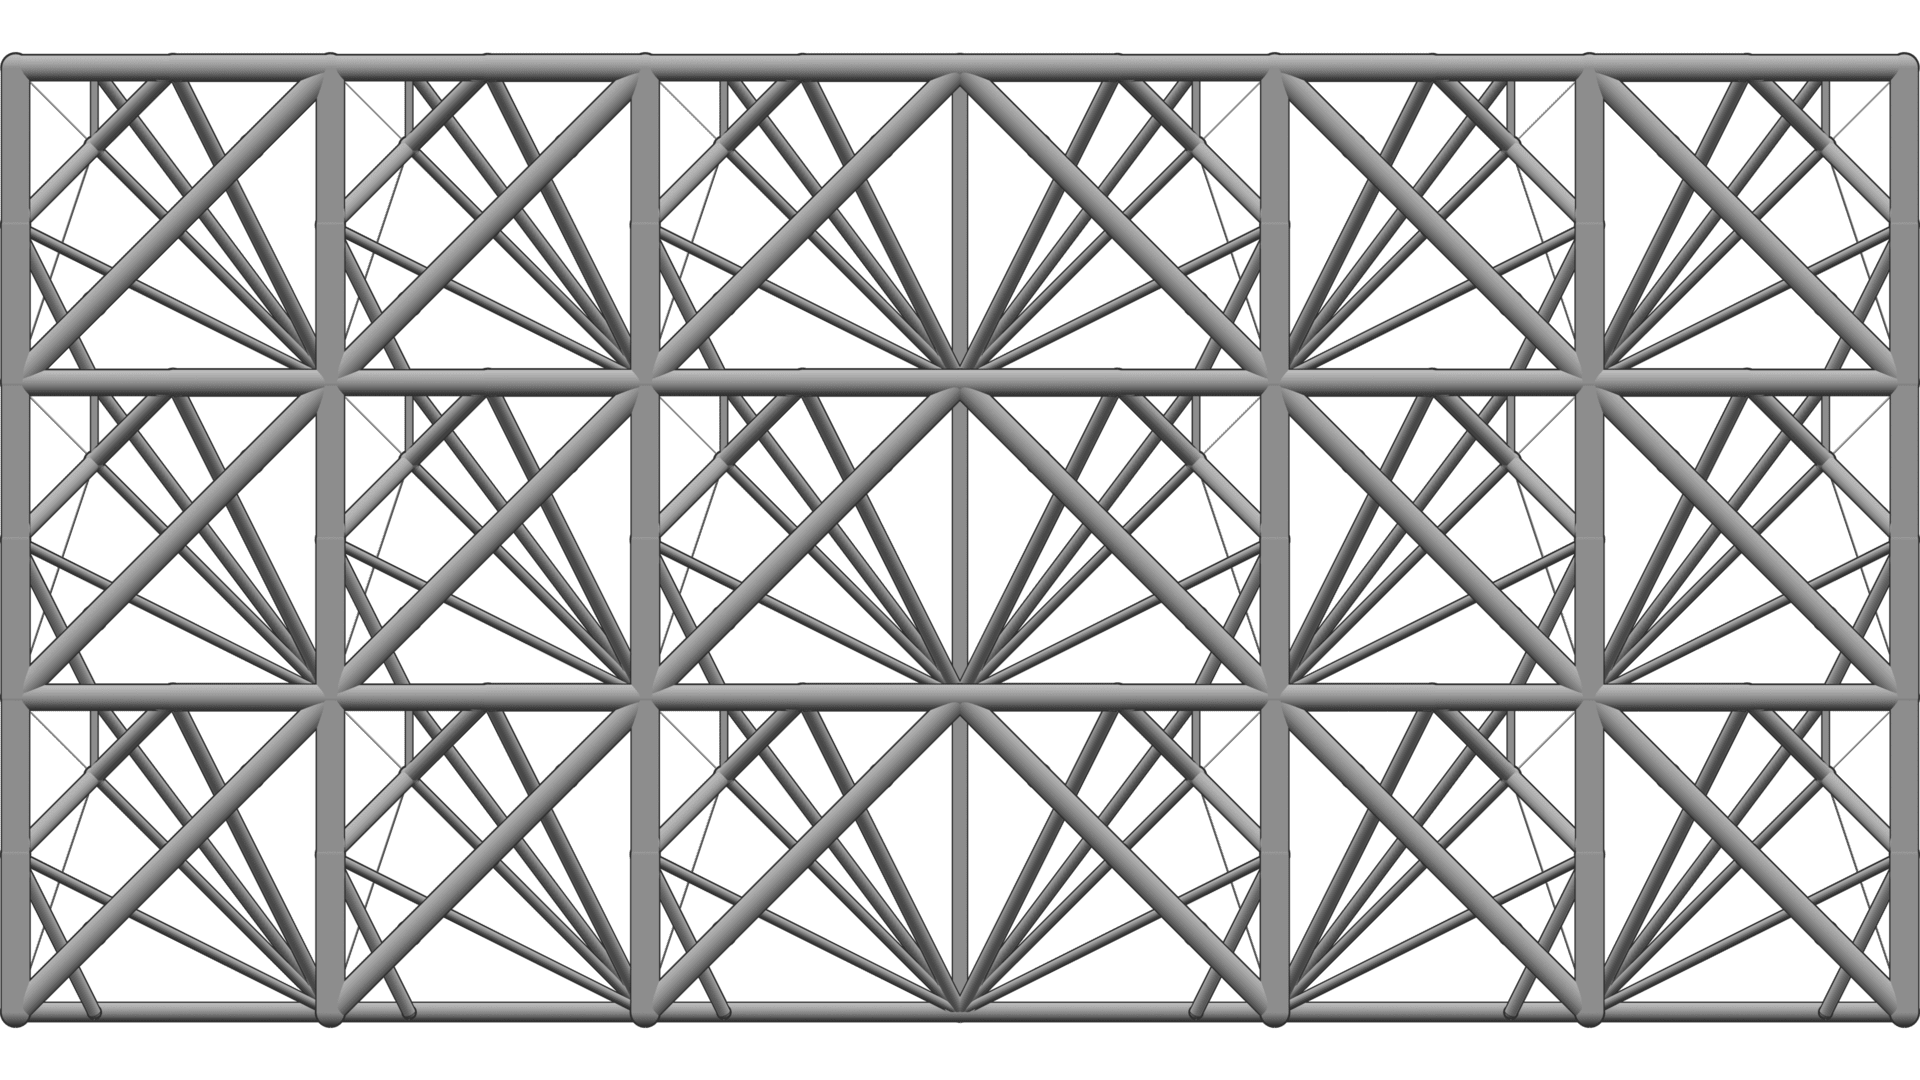
\includegraphics[width=0.23\linewidth]{figures/05_cellular_opt/00_module_complexity/6x2x3_5x5x5_XZ.png}}
    \hspace*{\fill}
    \caption{(a-d) (e-h)}
    \label{fig:05}
\end{figure*}

\begin{marginfigure}
    \centering
    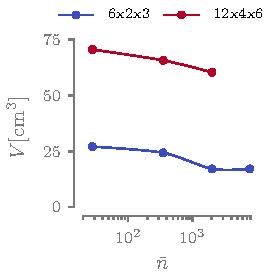
\includegraphics{figures/05_cellular_opt/00_module_complexity_tab/comp_tab.pdf}
    \caption{}
    \label{fig:05}
\end{marginfigure}

\begin{table*}
    \centering
    \small
    \begin{tabular}{lx{1.4cm}x{1.4cm}x{1.4cm}x{1.4cm}x{1.4cm}x{1.4cm}x{1.4cm}x{1.4cm}}
        \toprule
        \multirow{2}{*}{\textbf{Quantity}} & \multicolumn{4}{l}{6x2x3} & \multicolumn{3}{l}{12x4x6} \\ \cmidrule(lr){2-5} \cmidrule(lr){6-8} 
     & 2x2x2      & 3x3x3     &  4x4x4    &  5x5x5    &   2x2x2      & 3x3x3        & 4x4x4      \\
     &  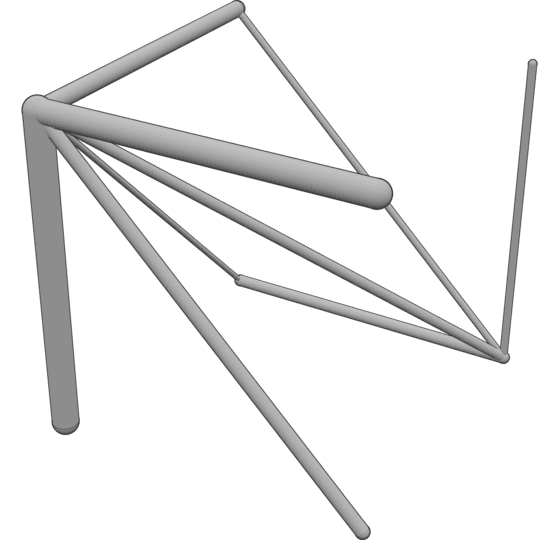
\includegraphics[width=1.3cm]{figures/05_cellular_opt/00_module_complexity_cell/6x2x3_2x2x2_c.png}    &  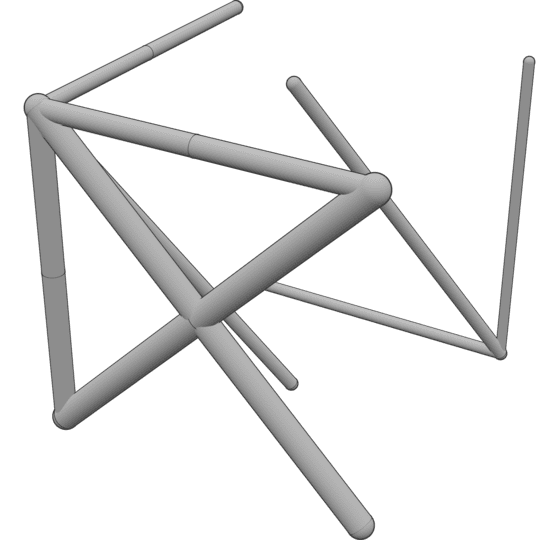
\includegraphics[width=1.3cm]{figures/05_cellular_opt/00_module_complexity_cell/6x2x3_3x3x3_c.png}    & 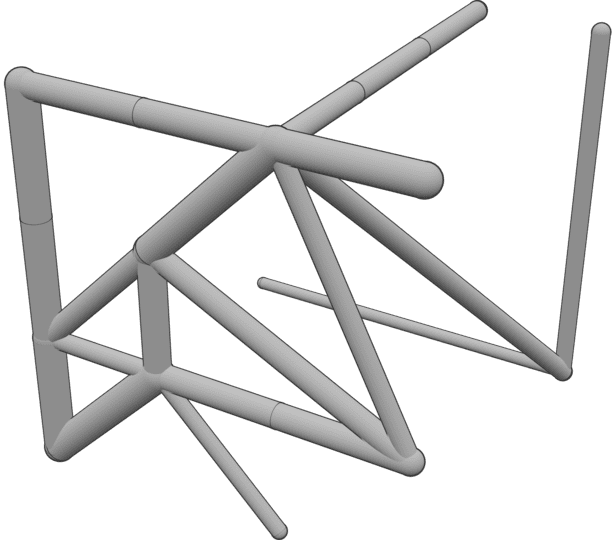
\includegraphics[width=1.3cm]{figures/05_cellular_opt/00_module_complexity_cell/6x2x3_4x4x4_c.png}     & 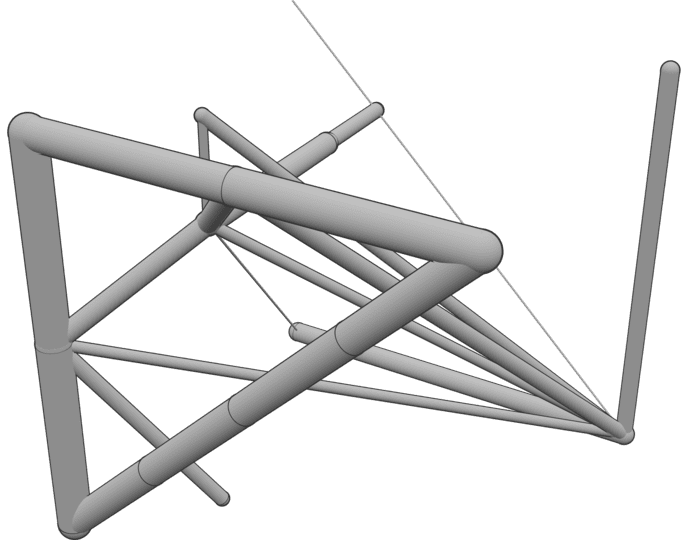
\includegraphics[width=1.3cm]{figures/05_cellular_opt/00_module_complexity_cell/6x2x3_5x5x5_c.png}     & 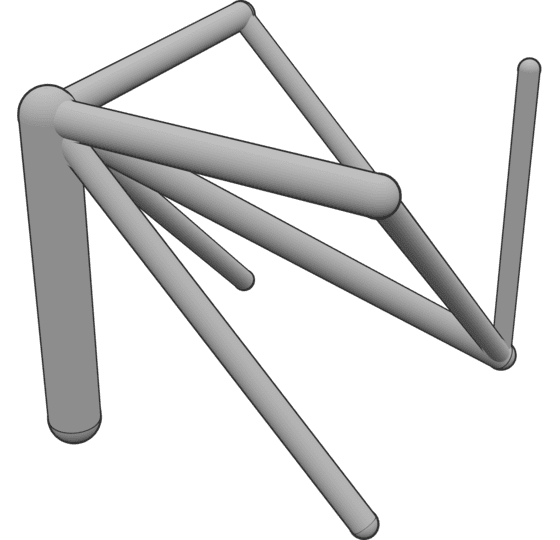
\includegraphics[width=1.3cm]{figures/05_cellular_opt/00_module_complexity_cell/12x4x6_2x2x2_c.png}        & 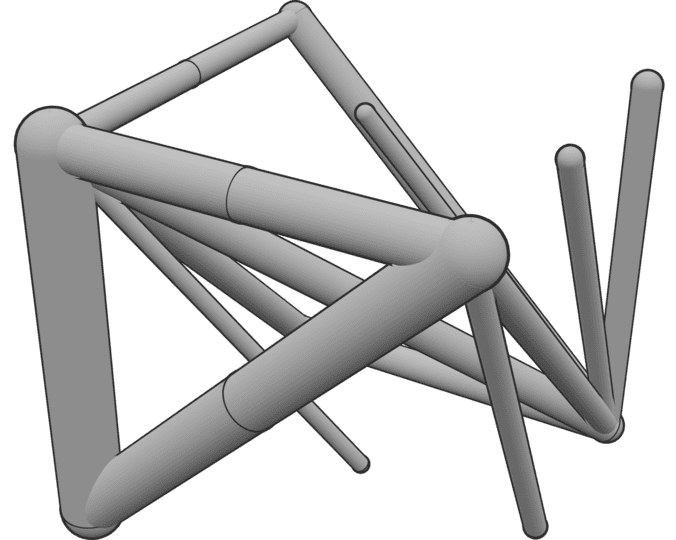
\includegraphics[width=1.3cm]{figures/05_cellular_opt/00_module_complexity_cell/12x4x6_3x3x3_c.png}   &  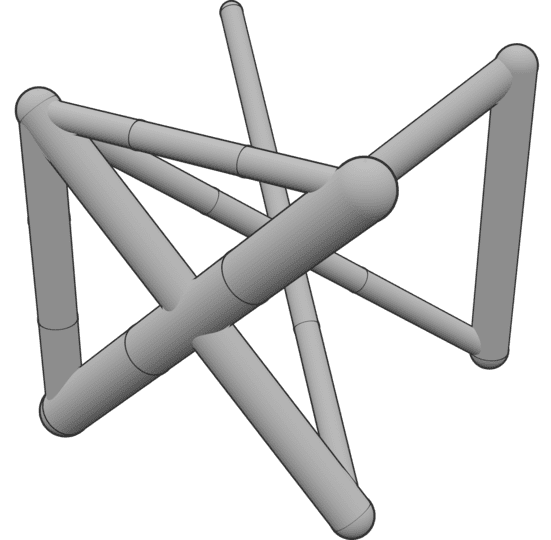
\includegraphics[width=1.3cm]{figures/05_cellular_opt/00_module_complexity_cell/12x4x6_4x4x4_c.png}      \\
    $\bar{n}_\text{opt}\;(\bar{n})$ &  9 (28) &   19 (351)   &  88  (2016)   &  88 (7750)    &   9 (28)   &    15 (351)        &   22   (2016)  \\
    $N_\text{sub}$           &    36  &   36   &   36   &   36   &    288     &   288      &    288    \\
    $N_\text{opt}\;(N_\text{el})$  &  324 (1008) &  468 (12636)   & 792  (72576)   & 792 (279000)     & 2592 (8064)     &   4320   (101088)       &  6336 (580608)     \\
    V [\unit{cm^3}] & 27.074 & 24.323     & 17.098     & 17.083     &  70.559    &  65.723       & 60.368       \\
    V [\unit{\percent}] &4.812&4.324&3.040&3.036&12.544&11.684&10.732        \\
    C [\unit{J}]      & 4.22     &   3.63   & 4.49     & 3.91     &   3.35      &  1.84       & 2.43       \\
    $a_\text{max}$ [\unit{mm^2}]      & 9.40     &   5.33   &   3.39   &  3.77    &  5.45       &   2.60      &   2.97    \\
    t        & \hms{0;0;6}  &  \hms{0;5;42} & \hms{0;14;20} & \hms{3;17;00} & \hms{0;0;48} & \hms{0;42;50} &  \hms{32;4;00}      \\ \bottomrule
    \end{tabular}
    \caption{}
    \label{tab:05_}
    \end{table*}

\todo{use blender to generate images}

\todo{check always the number of design variables, constraints and time}

\todo{devirendere i dati digesti, gare dei grafici di riepilogo delle cose interessanti. le tab servono da database ma non servono per spiegare}

\todo{different tables for every parametric study with iteration count}

\todo{name, table with number of candidates per module, number of subdomain and calculation time}

\todo{doe with calc time and volume}
Simply supported 3D beam

\todo{fai il doe}
we limit to cubic cell for semplicity
here are the outcomes

\begin{equation}
    a\:x_1^2+b\:x_2^2+c\:x_1x_2+d\:x_1+e\:x_2+f
\end{equation}

\begin{margintable}
    \small
    \centering
    \sisetup{table-auto-round}
    \begin{tabular}{cS[table-number-alignment = center, table-format = 1.2e1]}
    \toprule
    \textbf{Coeff.} & {\textbf{Value}} \\ \midrule
    $a$ & 9.002e-08    \\
    $b$ &  -1.022e-05   \\
    $c$ &  -1.770e-06   \\
    $d$ &  -2.644e-03   \\
    $e$ &   1.011e-01  \\
    $f$ &   2.881e+01  \\
    \bottomrule
    \end{tabular}
    \caption{Volume}
    \label{tab:05}
\end{margintable}

\begin{margintable}
    \small
    \centering
    \sisetup{table-auto-round}
    \begin{tabular}{cS[table-number-alignment = center, table-format = 1.2e1]}
    \toprule
    \textbf{Coeff.} & {\textbf{Value}} \\ \midrule
    $a$ & 1.547e-03    \\
    $b$ & -2.871e-04    \\
    $c$ &  2.896e-01   \\
    $d$ &  -2.084e+01   \\
    $e$ &  -5.543e+00   \\
    $f$ & 0    \\
    \bottomrule
    \end{tabular}
    \caption{Time}
    \label{tab:05}
\end{margintable}


\begin{figure*}
    \hspace*{\fill}
    \subcaptionbox{}{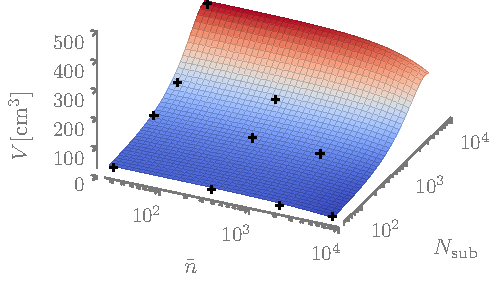
\includegraphics{figures/05_cellular_opt/00_doe_vol/doe_vol.pdf}}
    \hfill
    \subcaptionbox{}{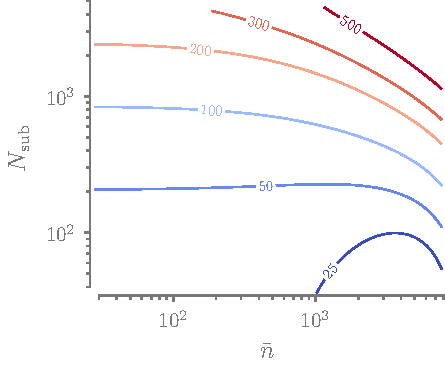
\includegraphics{figures/05_cellular_opt/00_doe_vol/doe_vol_cont.pdf}}
    \hspace*{\fill}
    \bigskip
    \hspace*{\fill}
    \subcaptionbox{}{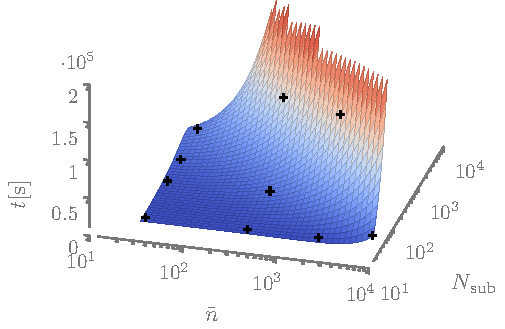
\includegraphics{figures/05_cellular_opt/00_doe_time/doe_time.pdf}}
    \hfill
    \subcaptionbox{}{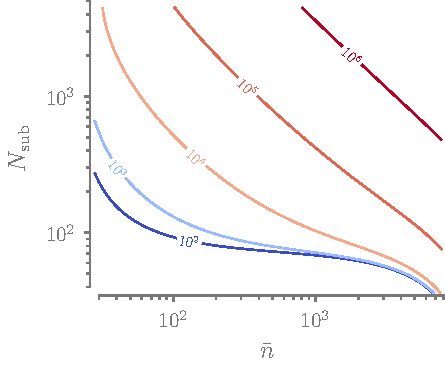
\includegraphics{figures/05_cellular_opt/00_doe_time/doe_time_cont.pdf}}
    \hspace*{\fill}
    \caption{limited to 500 and 2e5}
    \label{fig:05}
\end{figure*}

\subsection{Comparison with the optimized octet truss}

The \gls{tto} algorithm is here benchmarked against one of the most popular cell topologies present in the literature: the octet-truss (see Fig. xx). The octet-truss is a cell known for having very good effective mechanical properties that attain about half the theoretical values of the upper Hashi-Shtrikman bounds~\sidecite{deshpande_effective_2001}. 

To perform the benchmark, the wing box of Figure~xxis meshed using 44×4×1 octet-truss cells of 125 mm of edge size (see Fig. xx). The cross-sectional areas of the cell members are all equal. The section value is evaluated by performing a parametric optimization on this section value, constrained by stress and local buckling for every member of the structure. The optimization is performed using Altair OptiStruct.

\begin{marginfigure}
    \centering
    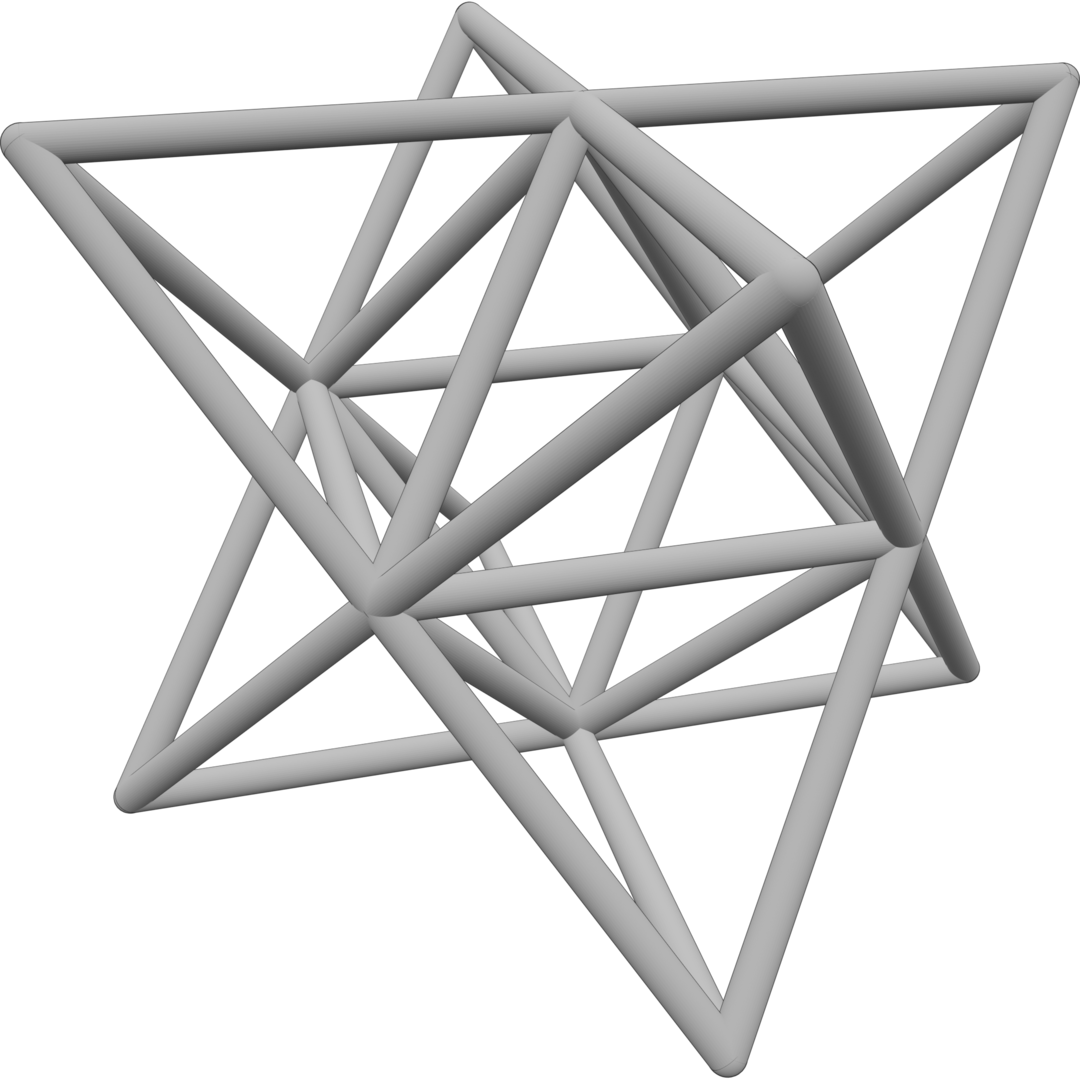
\includegraphics[width=0.7\linewidth]{figures/05_cellular_opt/00_octet/05_Cell__Topology_NLP_iso.png}
    \caption{}
    \label{fig:05}
\end{marginfigure}

\begin{figure*}
    \hspace*{\fill}
    \subcaptionbox{}{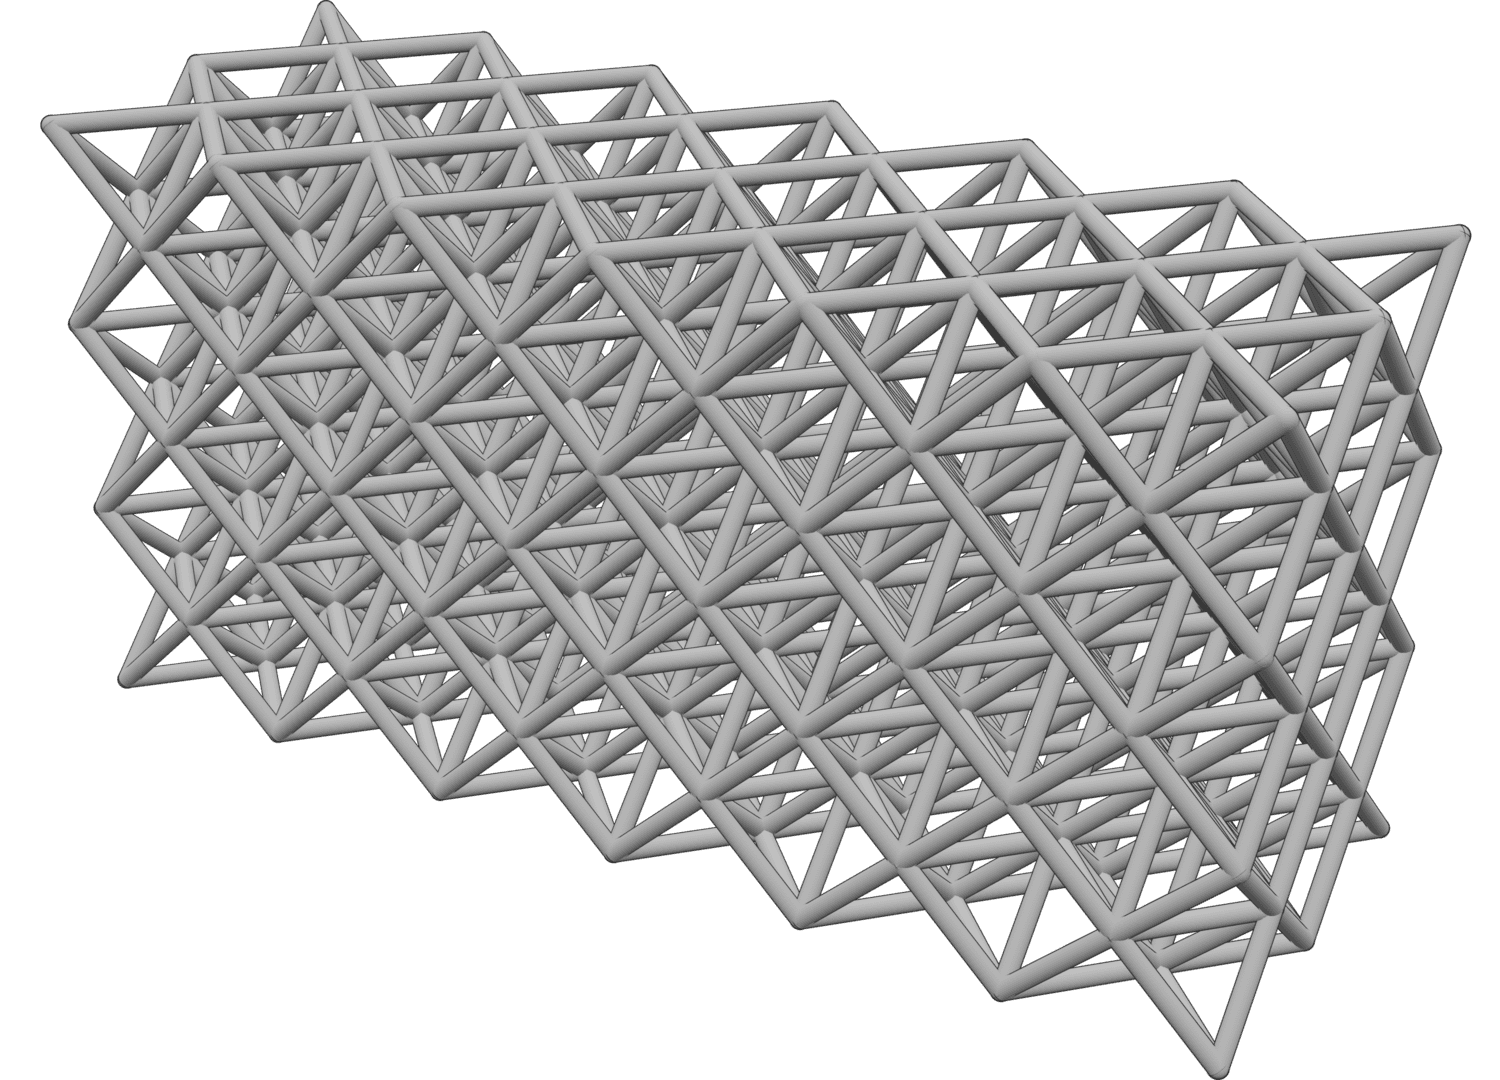
\includegraphics[width=0.46\linewidth]{figures/05_cellular_opt/00_octet_truss_comp_6/octet.png}}
    \hfill
    \subcaptionbox{}{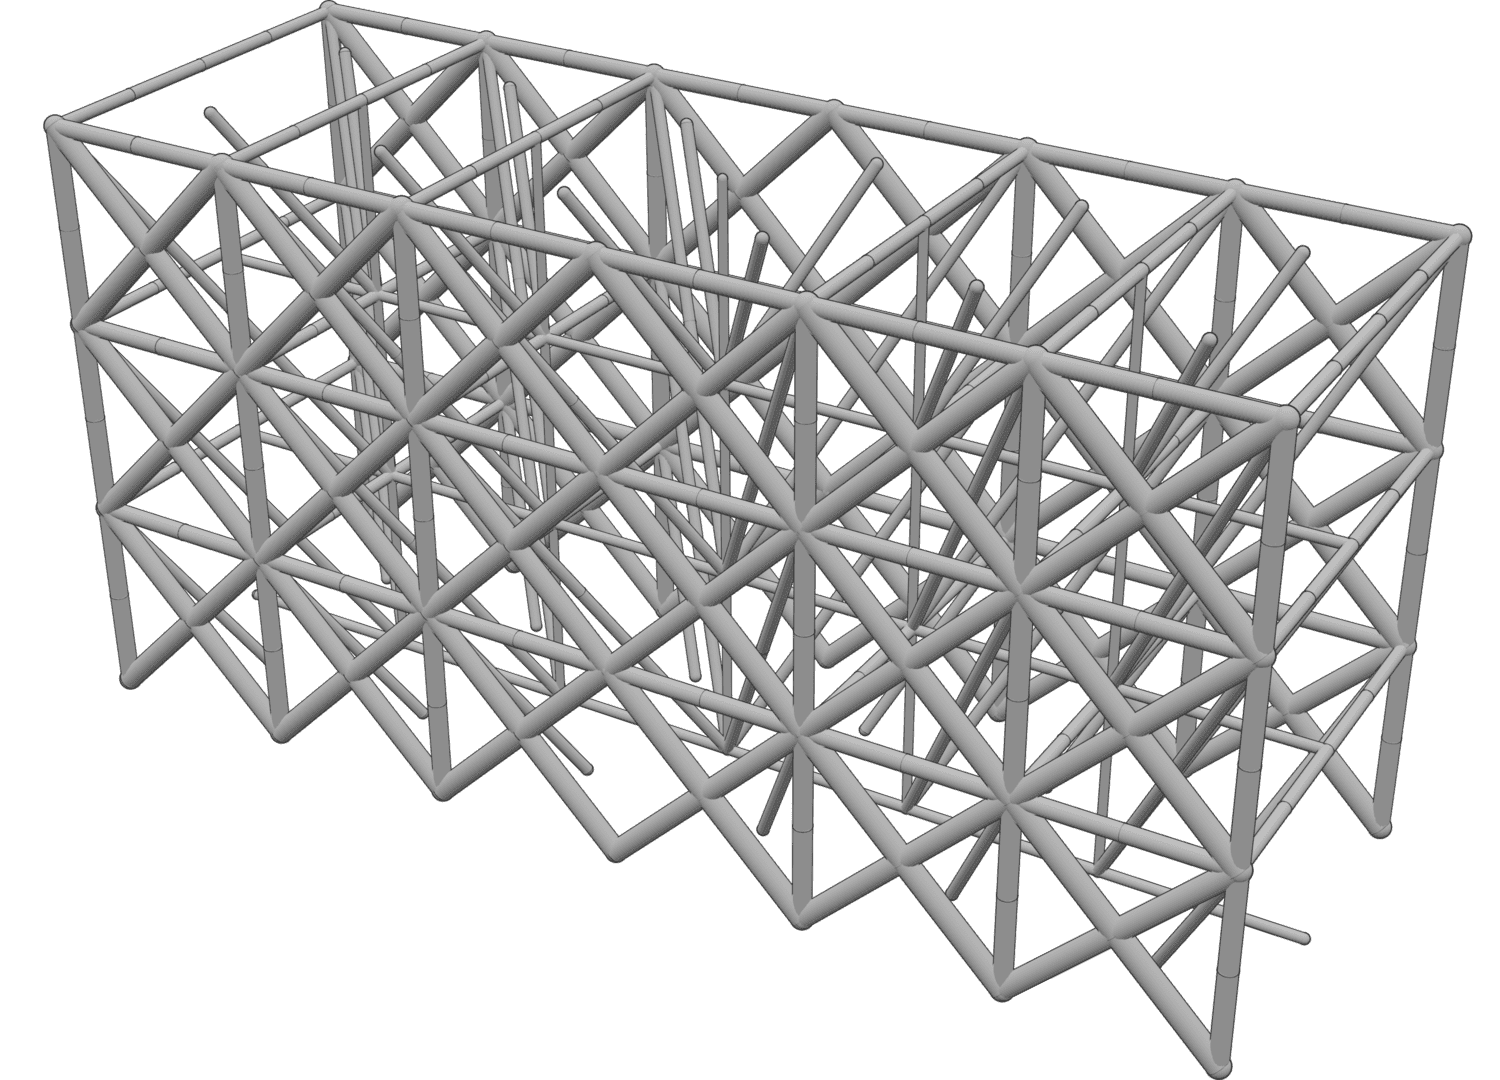
\includegraphics[width=0.46\linewidth]{figures/05_cellular_opt/00_octet_truss_comp_6/6x2x3_3x3x3.png}}
    \hspace*{\fill}
    \bigskip
    \hspace*{\fill}
    \subcaptionbox{}{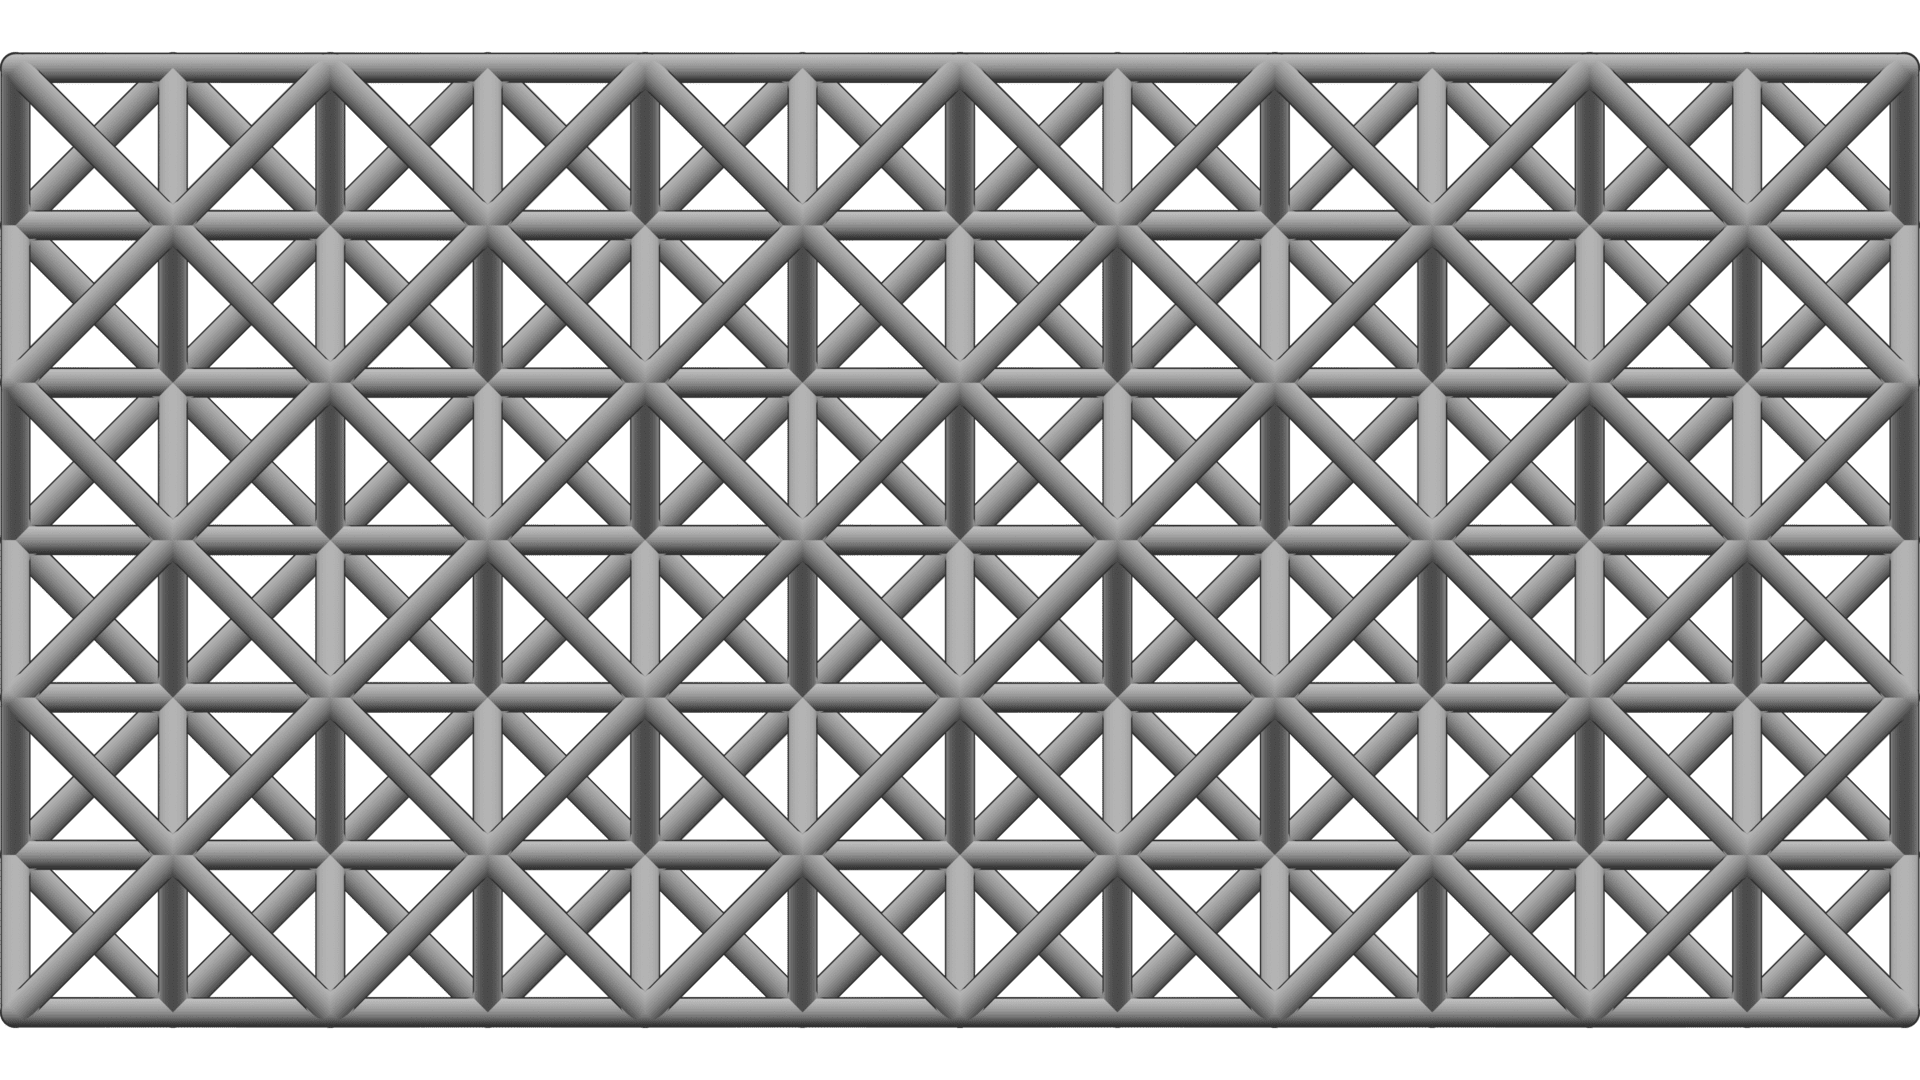
\includegraphics[width=0.46\linewidth]{figures/05_cellular_opt/00_octet_truss_comp_6/octet_XZ.png}}
    \hfill
    \subcaptionbox{}{\includegraphics[width=0.46\linewidth]{figures/05_cellular_opt/00_octet_truss_comp_6/6x2x3_3x3x3_XZ.png}}
    \hspace*{\fill}
    \caption{\todo{todo}}
    \label{fig:05}
\end{figure*}

\begin{figure*}
    \hspace*{\fill}
    \subcaptionbox{}{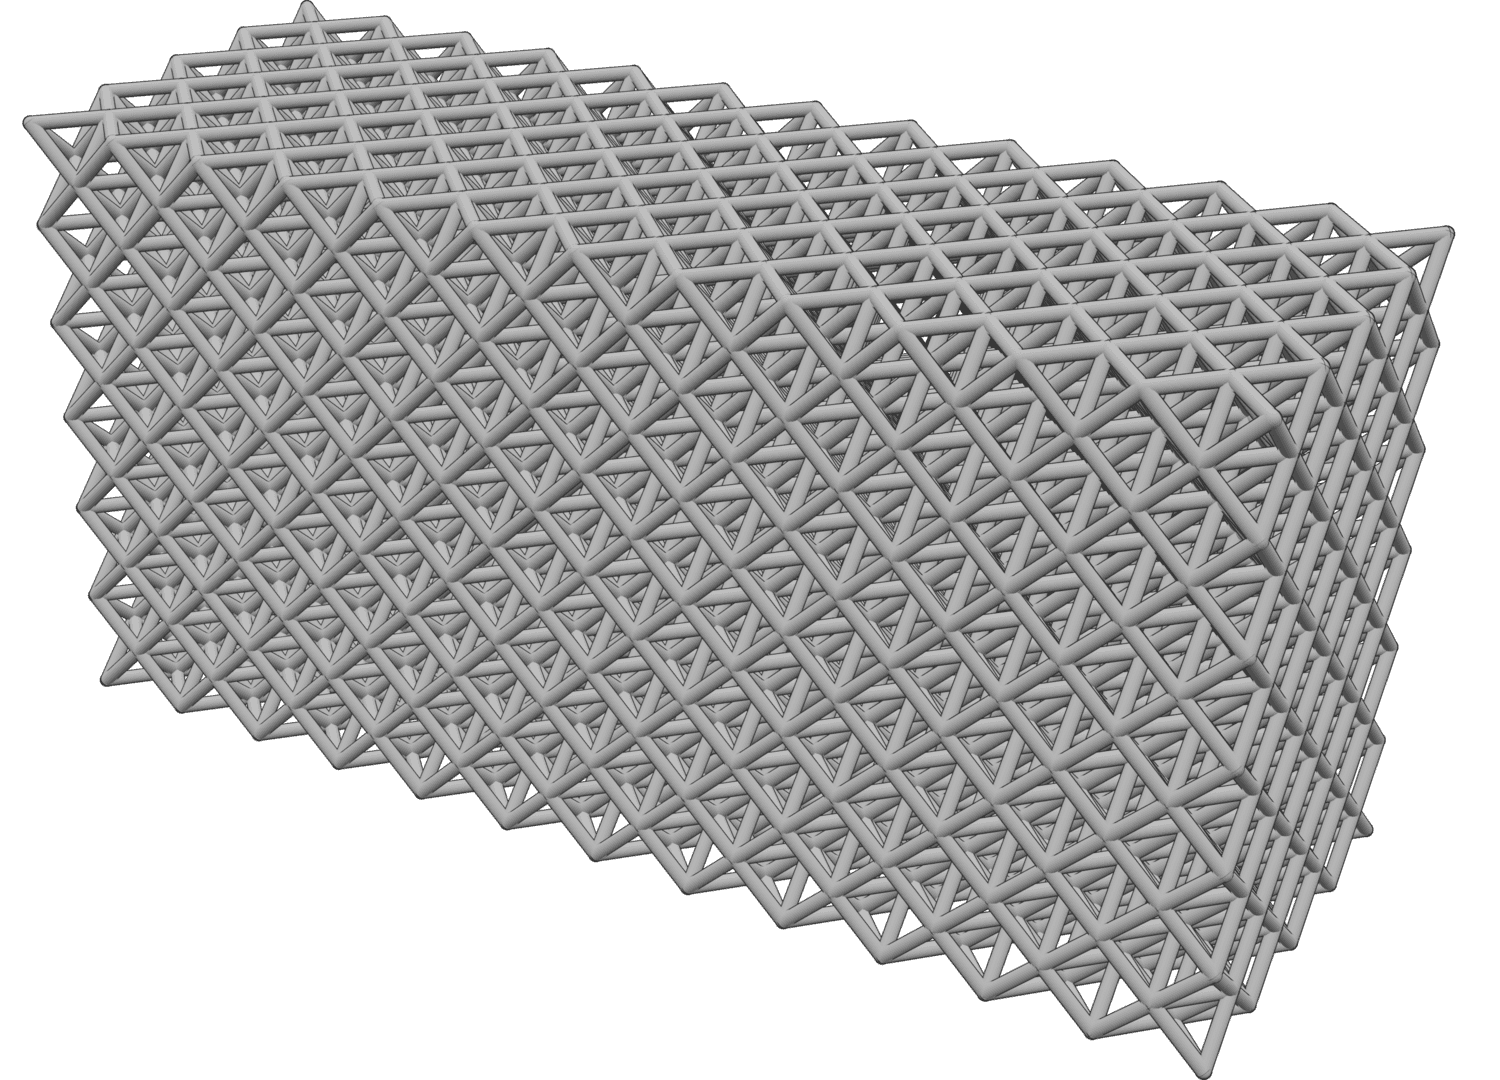
\includegraphics[width=0.46\linewidth]{figures/05_cellular_opt/00_octet_truss_comp_12/octet.png}}
    \hfill
    \subcaptionbox{}{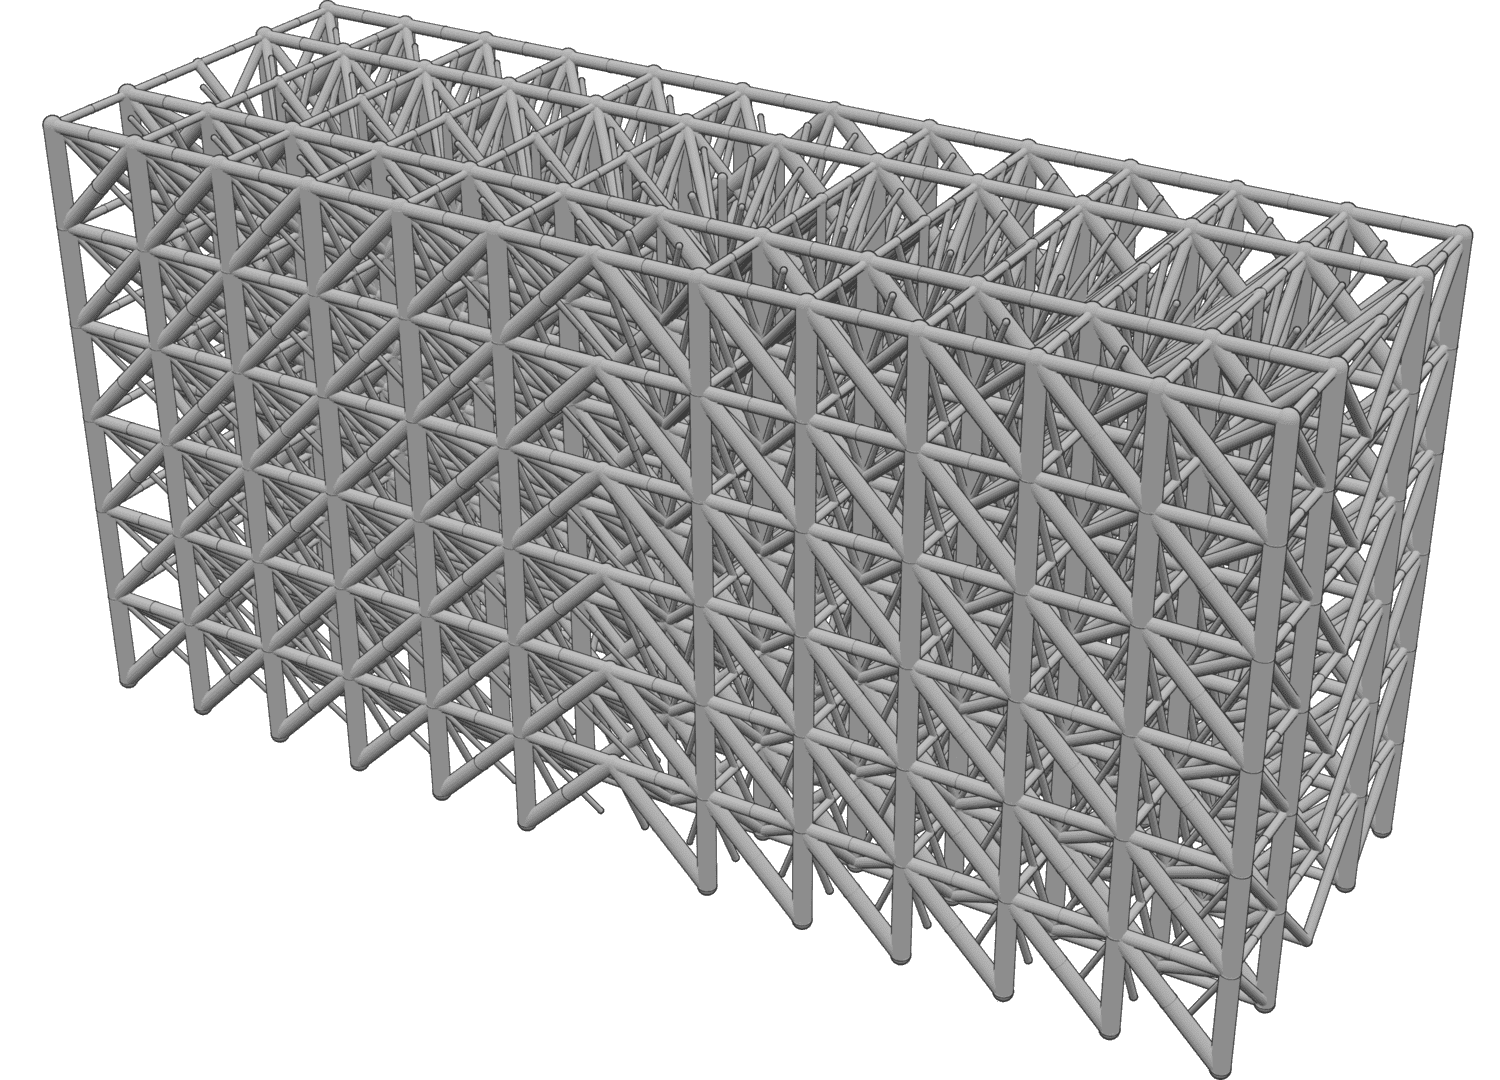
\includegraphics[width=0.46\linewidth]{figures/05_cellular_opt/00_octet_truss_comp_12/12x4x6_3x3x3.png}}
    \hspace*{\fill}
    \bigskip
    \hspace*{\fill}
    \subcaptionbox{}{\includegraphics[width=0.46\linewidth]{figures/05_cellular_opt/00_octet_truss_comp_12/octet_XZ.png}}
    \hfill
    \subcaptionbox{}{\includegraphics[width=0.46\linewidth]{figures/05_cellular_opt/00_octet_truss_comp_12/12x4x6_3x3x3_XZ.png}}
    \hspace*{\fill}
    \caption{\todo{todo}}
    \label{fig:05}
\end{figure*}

\begin{table}
    \centering
    \small
    \begin{tabular}{lx{1.4cm}x{1.4cm}x{1.4cm}x{1.4cm}}
        \toprule
        \multirow{2}{*}{\textbf{Quantity}}         &\multicolumn{2}{l}{6x2x3} & \multicolumn{2}{l}{12x4x6} \\ 
             \cmidrule(lr){2-3} \cmidrule(lr){4-5} 
     &Octet& 3x3x3      & Octet     &  3x3x3    \\
    $N_\text{sub}$       &36& 36&288&288   \\
    $N_\text{opt}\;(N_\text{el})$ &1008& 468 (12636)&7488&4320 (101088) \\
    V [\unit{cm^3}]& 65.752 & 24.323&121.038&65.723         \\
    V [\unit{\percent}] &11.692&4.324&21.524&11.684         \\
    C [\unit{J}]    &1.67&3.63&1.12&1.84         \\
    $a_\text{max}$ [\unit{mm^2}]    & 3.69 &  5.33&1.83&2.60         \\ \bottomrule
    \end{tabular}
    \caption{}
    \label{tab:05_}
    \end{table}

\subsection{Using multiple module's topologies}

this stuty suggest that we have here a compromise between volume (and then mass) and manufacturing complexity. we studyed till now the two extremities, the full modular and the monolithic structure. we want now to see what happens in between

\begin{figure}
    \centering
    \includegraphics[width=0.6\linewidth]{figures/05_cellular_opt/00_mutiple_bc/supported_3D_symm.pdf}
    \caption{}
    \label{fig:05}
\end{figure}

$\matr{H}=
\begin{bmatrix}
    1 & 0 & 0\\
    1 & 0 & 0\\
    1 & 0 & 0\\
    0 & 0 & 0\\
    0 & 1 & 0\\
    0 & 1 & 0\\
    0 & 1 & 0\\
    0 & 0 & 1\\
    0 & 0 & 1\\
    0 & 0 & 1\\
\end{bmatrix}$

show a picture that the design is more stressed compared to before

\begin{figure*}
    \centering
    \includegraphics{figures/05_cellular_opt/00_multiple_topology/support_sol.pdf}
    \caption{}
    \label{fig:05}
\end{figure*}

\begin{marginfigure}
    \centering
    \includegraphics[width=\linewidth]{figures/05_cellular_opt/00_multiple_tab/multi_tab.pdf}
    \caption{}
    \label{fig:05}
\end{marginfigure}

\begin{figure}
    \centering
    \includegraphics[width=\linewidth]{figures/05_cellular_opt/00_multiple_failure/mul_mech.pdf}
    \caption{\todo{todo}}
    \label{fig:05}
\end{figure}

\begin{table}
    \centering
    \small
    \begin{tabular}{lx{1.4cm}x{1.4cm}x{1.4cm}x{1.4cm}x{1.4cm}}
        \toprule
        \multirow{2}{*}{\textbf{Quantity}}   & 7x3x4 & \multicolumn{3}{l}{6x2x3 $N_\text{t}=3$} & 6x2x3 $N_\text{t}=1$ \\ \cmidrule(lr){2-2} \cmidrule(lr){3-5} \cmidrule(lr){6-6} 
     & --      & $t=0$    &  $t=1$    &  $t=2$    &   $t=0$       \\
     & --  &  \includegraphics[width=1.3cm]{figures/05_cellular_opt/00_multiple_cell/05_Cell_000_Topology_NLP_iso.png}    & \includegraphics[width=1.3cm]{figures/05_cellular_opt/00_multiple_cell/05_Cell_001_Topology_NLP_iso.png}     & --  & \includegraphics[width=1.3cm]{figures/05_cellular_opt/00_module_complexity_cell/6x2x3_3x3x3_c.png} \\
     $\bar{n}_\text{opt}\;(\bar{n})$ &1984 &   10 (351)   &  18  (351)       &   -- (351)   &    19 (351)  \\
    $N_\text{sub}$           &    1  & \multicolumn{3}{c}{36}   &    36    \\
    $N_\text{opt}\;(N_\text{el})$ &20 (1984) &  \multicolumn{3}{c}{336 (12636)}     &  468 (12636)     \\
    V [\unit{cm^3}]&9.907 &  \multicolumn{3}{c}{12.032}   & 24.323       \\
    V [\unit{\percent}] &1.761& \multicolumn{3}{c}{2.139} &4.324       \\
    C [\unit{J}]    &3.71     & \multicolumn{3}{c}{6.14}  & 3.63       \\
    $a_\text{max}$ [\unit{mm^2}]   &37.61   &  \multicolumn{3}{c}{7.13}   &   5.33    \\
    t     &\hms{0;0;4}  & \multicolumn{3}{c}{\hms{00;3;22}} &  \hms{00;5;42}      \\ \bottomrule
    \end{tabular}
    \caption{}
    \label{tab:05_}
    \end{table}


\section{Conclusion}
It's all part of our effort to strike a balance between mechanical performance and the ease of manufacturing, a topic we'll delve into further in the upcoming chapters.